% !TEX program = pdflatex
\documentclass{ieeeaccess}
\usepackage{cite}
\usepackage{amsmath,amssymb,amsfonts}
\usepackage{graphicx}
\usepackage{booktabs}
\usepackage{multirow}
\usepackage{xcolor}
\usepackage{url}
\usepackage{textcomp}
\usepackage{array}
\usepackage{placeins}

\renewcommand{\arraystretch}{1.2}

\graphicspath{{figures/}}

% Custom commands
\newcommand{\Hpre}{H_{\text{pre}}}
\newcommand{\Hpost}{H_{\text{post}}}
\newcommand{\Htl}{H_{\text{tl}}}

\begin{document}
\history{Date of publication xxxx 00, 0000, date of current version xxxx 00, 0000.}
\doi{10.1109/ACCESS.2026.DOI}

\title{Decoded Entropy Is Not One Signal: Pre- and Post-RMSNorm Projections Yield Non-Equivalent Measurements in RMSNorm-Based Decoder LMs}

\author{\uppercase{Sungmoon Park}\authorrefmark{1} and \uppercase{Jinhong Yang}\authorrefmark{2}}

\address[1]{Department of Healthcare IT, Inje University, Gimhae 50834, Republic of Korea (e-mail: qkrtjdans55@oasis.inje.ac.kr)}
\address[2]{Department of Healthcare IT, Inje University, Gimhae 50834, Republic of Korea (e-mail: jinhong@inje.ac.kr)}

\tfootnote{This work was supported by the Korea Institute for Advancement of Technology (KIAT) grant funded by the Korea government (Ministry of Trade, Industry and Energy) through the International Cooperation in Industrial Technology program (Project Number: P0026190) and Institute of Information \& Communications Technology Planning \& Evaluation (IITP)-Innovative Human Resource Development for Local Intellectualization program grant funded by the Korea government (MSIT) (IITP-2026-RS-2024-00436773).}

\markboth
{Park and Yang: Decoded Entropy Is Not One Signal}
{Park and Yang: Decoded Entropy Is Not One Signal}

\corresp{Corresponding author: Jinhong Yang (e-mail: jinhong@inje.ac.kr).}

\begin{abstract}
Layerwise decoded entropy---the Shannon entropy of intermediate hidden states projected to vocabulary space---is increasingly used as an internal diagnostic in decoder language models (LMs) that employ root mean square layer normalization (RMSNorm), yet whether the projection is applied before or after the final RMSNorm has not been consistently specified. We empirically quantify the consequences of this implementation choice in three 7--8B instruction-tuned decoder LMs (Qwen2.5-7B, Llama-3-8B, Mistral-7B). Pre-normalization entropy ($\Hpre$) and post-normalization entropy ($\Hpost$) are non-equivalent measurements: $\Hpre$ is mathematically scale-sensitive by construction (softmax temperature effect) and our interventions confirm that its empirical magnitude is large---unit-normalizing hidden states collapses $\Hpre$ toward maximal entropy in all three families---whereas $\Hpost$ is largely scale-invariant in middle and late layers. This non-equivalence has two practical consequences in the tested settings: (i)~simple scale baselines (logit standard deviation, hidden-state norm) from a single forward pass match or exceed single-layer entropy for correctness discrimination, offering a compute-efficient internal confidence signal; (ii)~$\Hpre$ and $\Hpost$ yield different per-layer discrimination landscapes and classifier choice alone shifts the apparent area under the receiver operating characteristic curve (AUROC) by up to +0.17, so reported findings depend on which variant is used. All reported quantities are decoder-dependent diagnostic measurements under the raw logit lens and should not be interpreted as direct readouts of latent model belief. As illustrative context, we note cross-paper variation in normalization reporting and recommend that future studies specify the normalization point, include direct scale baselines, and report classifier and token-position choices.
\end{abstract}

\begin{keywords}
Large language models, logit lens, layerwise entropy, RMSNorm, measurement non-equivalence, uncertainty estimation, scale sensitivity.
\end{keywords}

\titlepgskip=-15pt

\maketitle

%===============================================================================
\section{Introduction}
\label{sec:introduction}

\PARstart{I}{n} the three root mean square layer normalization (RMSNorm)-based decoder language models (LMs) studied here, layerwise decoded entropy is not one measurement. Pre-normalization entropy ($\Hpre$) and post-normalization entropy ($\Hpost$)---computed from the same hidden state at a given layer---are non-equivalent quantities with different invariance properties, different optimal layers, and different downstream analytical conclusions. Our contribution is not to claim an unexpected phenomenon in principle---the softmax temperature effect that underlies this distinction is well known---but to show that this implementation choice is large enough in realistic evaluation pipelines to change empirical conclusions, and to quantify the resulting consequences across three 7--8B instruction-tuned decoder LMs.

Layerwise decoded entropy---the Shannon entropy computed from intermediate hidden states projected to vocabulary space---has attracted growing attention as an internal diagnostic \cite{ali2025entropylens, ghandeharioun2024patchscopes, kossen2024seps}. However, an implementation choice with measurement consequences has not been consistently specified: in transformer architectures employing RMSNorm, entropy computed before versus after the final normalization step may measure qualitatively different quantities---yet existing work is inconsistent on which is used (see illustrative audit in Section~\ref{sec:implications}). RMSNorm removes radial scale from hidden states, and if pre-normalization entropy is dominated by that scale, then researchers using logit-lens entropy without normalization may be reporting hidden-state magnitude rather than distributional content.

We ask whether layerwise decoded entropy remains a single measurement, or whether the normalization point splits it into distinct quantities.

We define $\Hpre$ = entropy of $\text{softmax}(W h_l)$ and $\Hpost$ = entropy of $\text{softmax}(W \cdot \text{RMSNorm}(h_l))$. Both are diagnostic projections---applying the final-layer decoder to intermediate representations that were not designed to be decoded at that point (Fig.~\ref{fig:overview}). Decomposing $h_l = r_l u_l$ into radial magnitude $r_l$ and direction $u_l$, $\Hpre$ responds to hidden-state magnitude because pre-norm logits scale linearly with $r_l$, acting as an implicit temperature. $\Hpost$, computed after RMSNorm removes radial scale, is largely invariant to magnitude rescaling---except in low-norm early layers where the implementation's epsilon term breaks exact invariance. We verify lens faithfulness caveats for these diagnostic projections in Section~\ref{sec:decoder}.

This distinction has two practical consequences:

\begin{enumerate}
\item \textbf{Simple scale baselines offer a compute-efficient internal confidence signal.} In all tested post-generation settings, scale-correlated baselines (logit standard deviation, hidden-state norm) from a single forward pass match or exceed single-layer $\Hpre$ for correctness discrimination. Adding $\Hpre$ to these baselines leaves little incremental utility (95\% confidence intervals (CIs) for the change in area under the receiver operating characteristic curve (delta-AUROC) include zero in all four logit\_std+$\Hpre$ comparisons; one full-feature comparison on Mistral yields a nominal-level positive delta). The best internal-layer signal exceeds final-output entropy by +0.09 to +0.22 AUROC, and this advantage holds under greedy decoding (Section~\ref{sec:predictive}).

\item \textbf{Reported findings depend on normalization point, classifier, and protocol.} The best layer, sign direction, and even which entropy variant is more useful all vary across model family, task, and evaluation protocol. $\Hpost$ exhibits cross-family sign reversal. Switching the Entropy-Lens classifier from $k$-NN to logistic regression (LR) changes AUROC by up to +0.17. No universal optimal layer emerges under our protocol (Sections~\ref{sec:where} and \ref{sec:decoder}).
\end{enumerate}

Our contributions are:

\begin{itemize}
\item \textbf{C1. Measurement non-equivalence quantification.} We quantify how the normalization point changes decoded-entropy behavior in three tested 7--8B RMSNorm-based instruction-tuned decoder LMs. Via unit-norm removal and alpha-sweep interventions, we show that $\Hpre$ is mathematically scale-sensitive by construction and that this sensitivity has large empirical magnitude, whereas $\Hpost$ is largely scale-invariant outside low-norm early layers under the $\epsilon$-regularized RMSNorm implementation. The normalization point therefore changes what decoded entropy emphasizes under the raw logit-lens projection---a confound that has not been consistently controlled for in the works surveyed in Section~\ref{sec:implications} (Section~\ref{sec:what}).

\item \textbf{C2. Practical consequence under matched evaluation.} Under held-out and reproduced evaluation protocols, normalization point and classifier choice substantially change analytical outcomes: $\Hpre$ and $\Hpost$ yield different per-layer AUROC landscapes, scale-correlated baselines match or exceed single-layer entropy for correctness discrimination in the tested conditions, classifier choice shifts apparent AUROC by up to +0.17, and the selective-prediction top-ranked model changes when $\Hpre$ is replaced by $\Hpost$. Profile-level scale redundancy largely persists under greedy decoding. A borderline exception on Mistral (+0.016) does not survive Bonferroni correction across the eight primary tests (Sections~\ref{sec:predictive}, \ref{sec:decoder}).

\item \textbf{C3. Illustrative audit and reporting recommendations.} We document inconsistent normalization specification in a representative (not systematic) survey of prior decoded-entropy work and provide a six-item reporting checklist. The audit documents cross-paper variation in specification practices, not invalidity---we do not claim that any specific prior conclusion is incorrect without matched re-evaluation (Sections~\ref{sec:implications}, \ref{sec:recommendations}).
\end{itemize}

\begin{figure*}[!t]
\centering
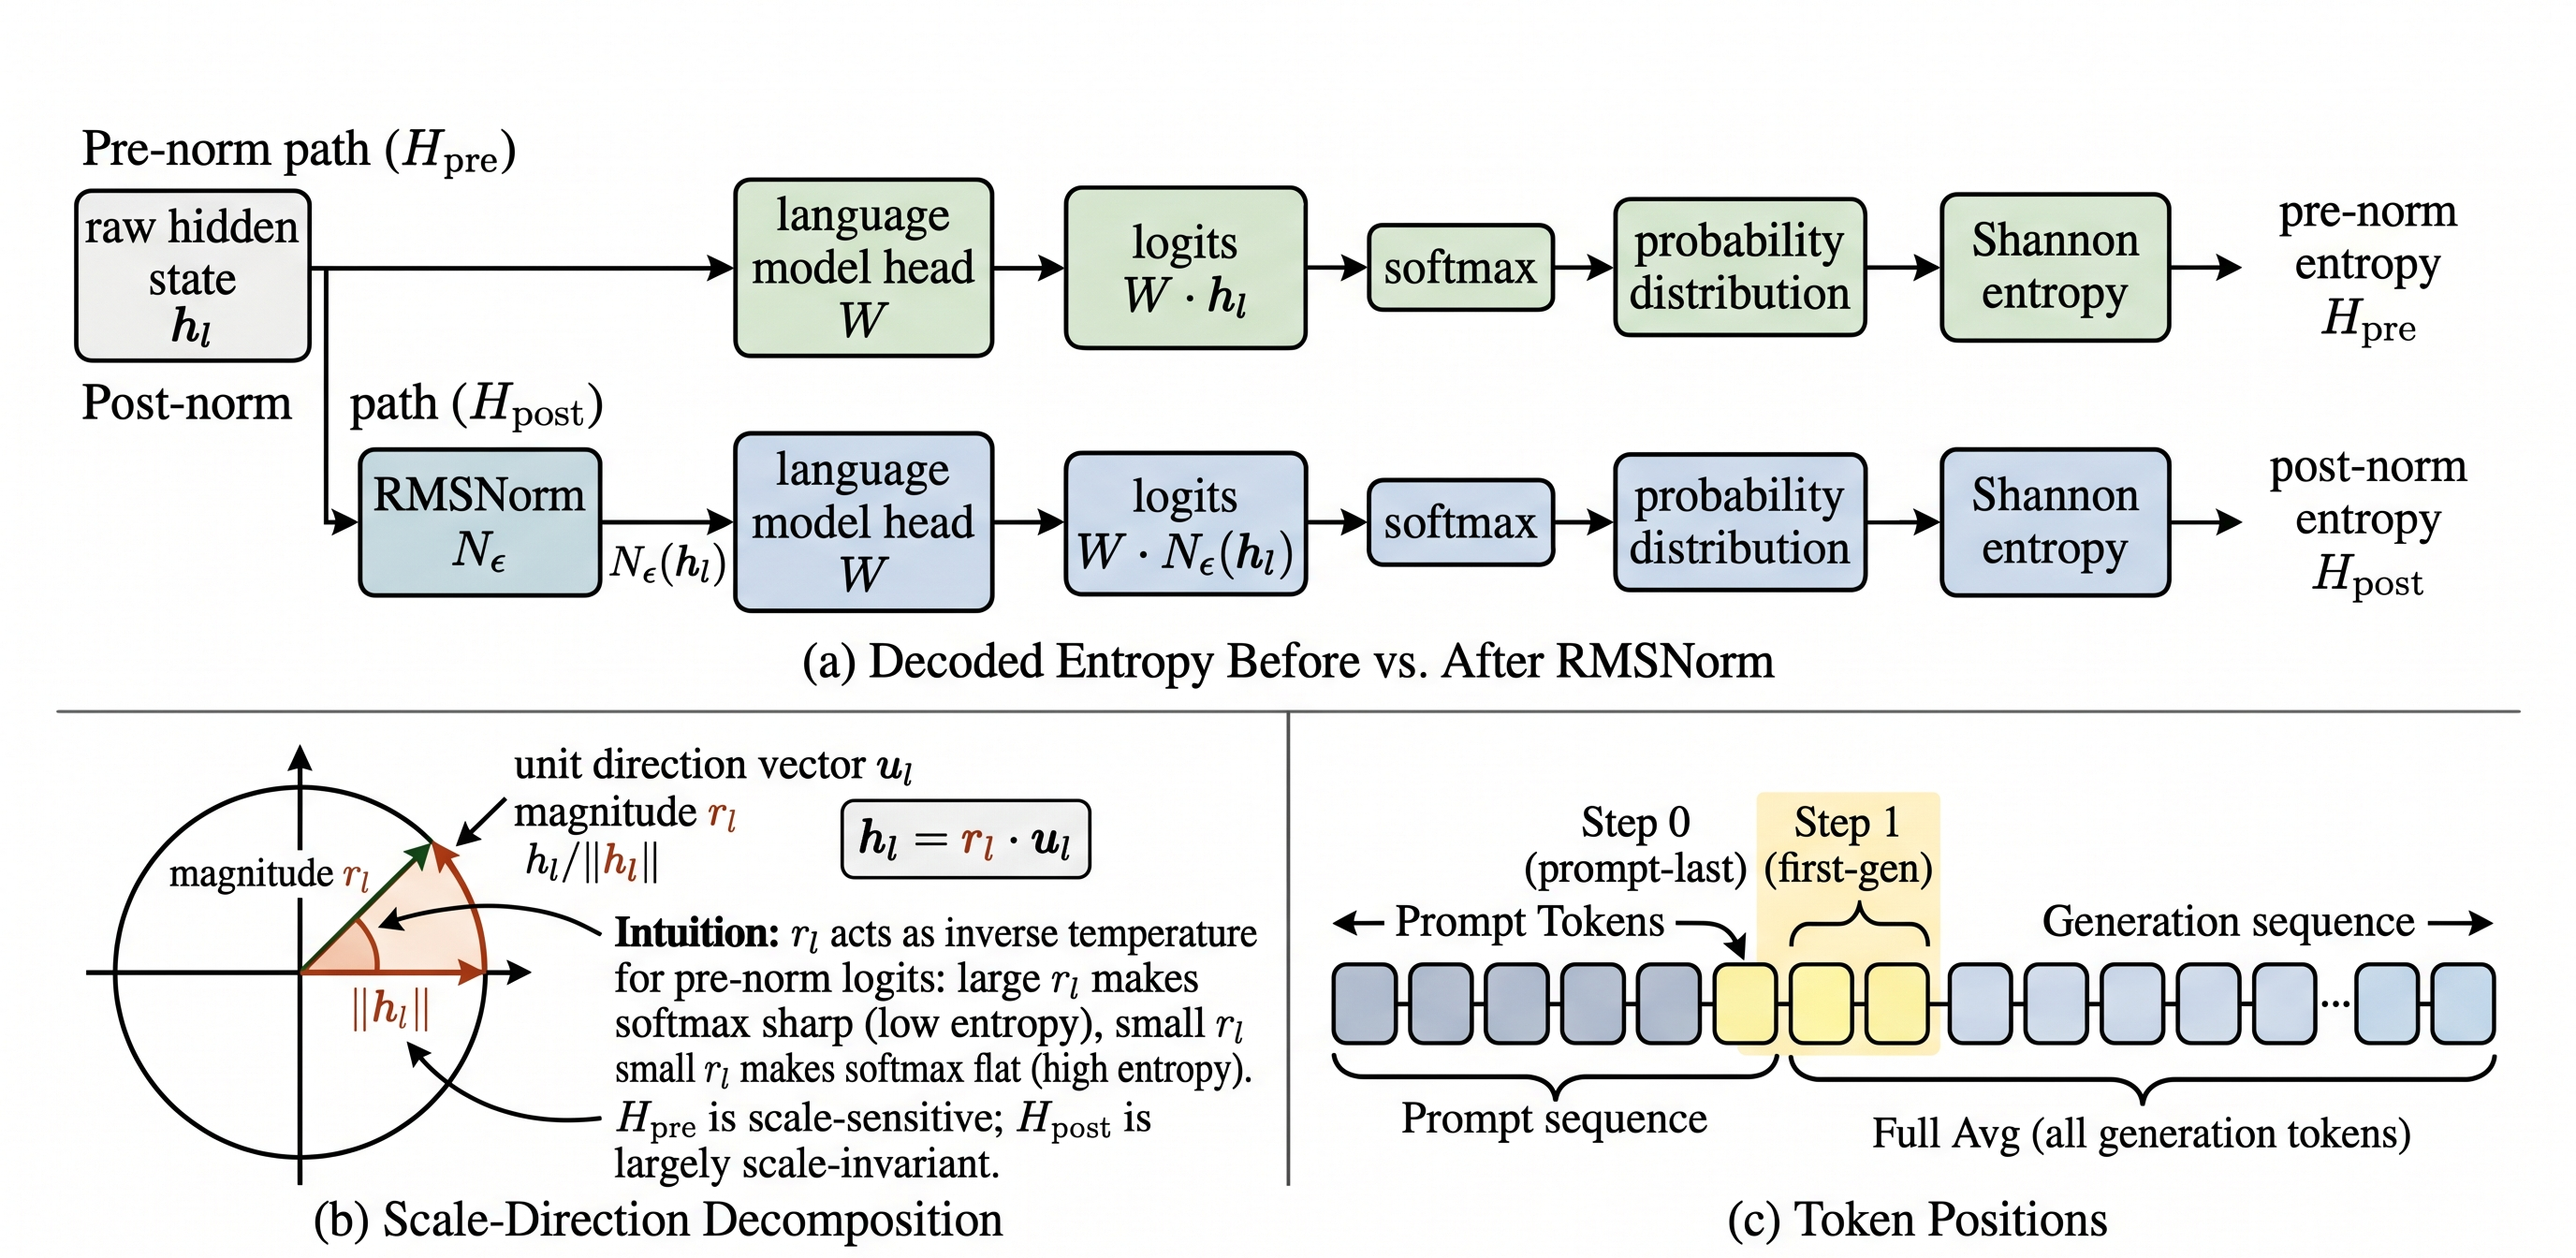
\includegraphics[width=\textwidth]{fig1.png}
\caption{Conceptual overview. (a)~$\Hpre$ applies the language model head $W$ directly to intermediate hidden states $h_l$, while $\Hpost$ first applies the final RMSNorm. (b)~Decomposing $h_l = r_l u_l$ into radial magnitude $r_l$ and unit direction $u_l$: $r_l$ acts as an inverse temperature for pre-norm logits. (c)~Three token positions used throughout: Step~0 (prompt-last), Step~1 (first generated token), and Full Average (all generation tokens).}
\label{fig:overview}
\end{figure*}

This paper is an empirical measurement study of how the normalization point changes the interpretation of layerwise decoded entropy. Our claims are limited to RMSNorm-based 7--8B decoder LMs and the evaluation settings studied here, centered on Massive Multitask Language Understanding (MMLU) \cite{hendrycks2021mmlu}, competition\_math \cite{hendrycks2021math}, and matched auxiliary extensions. We do not test LayerNorm-based architectures, substantially larger models, or open-ended long-form generation tasks, so those cases should be treated as open empirical questions rather than implied generalizations. Our evaluation uses post-generation diagnostics (entropy computed from generated-token hidden states); the findings do not directly address pre-generation uncertainty estimation.

\textbf{Reader roadmap.} Primary evidence consists of three components: scale interventions (Section~\ref{sec:what}), held-out consequence analyses (Section~\ref{sec:predictive}), and normalization/classifier sensitivity analyses (Section~\ref{sec:decoder}). Token-position ablations (Section~\ref{sec:where}), Tuned Lens controls, protocol-matched reproductions, and the illustrative literature audit are robustness or contextual analyses and should be interpreted accordingly. Section~\ref{sec:related} reviews related work. Section~\ref{sec:definitions} defines $\Hpre$/$\Hpost$ and the evaluation protocol. Section~\ref{sec:discussion} discusses implications, limitations, and reporting recommendations (C3). Section~\ref{sec:conclusion} concludes.


%===============================================================================
\section{Related Work}
\label{sec:related}

\subsection{Layerwise Decoding and Entropy in LLMs}

The Logit Lens (LL) \cite{nostalgebraist2020logitlens} projects intermediate hidden states to vocabulary space via the language model head, enabling layer-by-layer inspection of evolving predictions. The Tuned Lens (TL) \cite{belrose2023tuned} improves upon this with learned affine translators, reducing representational drift; Belrose et al. explicitly define the logit lens with LayerNorm included. Geva et al. \cite{geva2022transformer} analyze how feed-forward layers promote concepts in vocabulary space, explicitly omitting LayerNorm from their projection and checking in an appendix that this omission does not substantially affect top-token interpretations. This finding is expected: scaling a hidden state $h$ by a positive factor $\alpha$ does not change $\arg\max(Wh)$, because the ranking of logit values is preserved under positive scaling. However, entropy is not rank-based---it depends on the full probability distribution, which changes under scaling because $\text{softmax}(\alpha Wh)$ treats $\alpha$ as an inverse temperature. Our alpha-sweep experiments (Section~\ref{sec:what}) confirm this: across three model families, scaling hidden states by factors of 0.25--4.0 produces substantial $\Hpre$ variation, reaching 0.924 in Qwen middle layers (vs.\ 0.008 for Llama and 0.0005 for Mistral). Top-token identity is analytically invariant under positive scaling because $\arg\max(\alpha Wh) = \arg\max(Wh)$ for $\alpha > 0$. Thus, Geva et al.'s finding that normalization does not affect top-token interpretation does not extend to entropy: the two quantities are sensitive to different properties of the logit distribution.

Entropy-Lens \cite{ali2025entropylens} studies entropy dynamics of logit-lens probabilities across layers to characterize expansion and pruning decision strategies; when $k$-NN is used, it is framed as a diagnostic probe rather than a proposed predictive model. DoLa \cite{chuang2024dola} contrasts logit distributions between early and late layers to improve factuality, projecting intermediate hidden states through the vocabulary head without specifying normalization. SimLens \cite{ma2025simlens} improves intermediate-layer decoding accuracy by eliciting predictions with one additional token, addressing lens drift at early layers.

Post-Logit-Lens work does not establish a single superiority ordering. Instead, improvements fall along at least three non-equivalent axes. \textit{Faithful same-object decoders} such as Tuned Lens \cite{belrose2023tuned} and learned linear shortcuts \cite{yomdin2024jump}---the latter reporting 15--40\% accuracy gains over identity projection in prediction estimation---improve fidelity to later-layer representations. \textit{Expressive decoding frameworks} such as Patchscopes \cite{ghandeharioun2024patchscopes} and Future Lens \cite{pal2023futurelens} broaden what can be extracted from a single hidden state, including subsequent-token predictions. \textit{Task-specific decoders} such as DoLa \cite{chuang2024dola} and SimLens \cite{ma2025simlens} target inference-time factuality or single-token early-exit utility rather than generic full-vocabulary faithfulness. \textit{Gradient-based approaches} such as the Backward Lens \cite{katz2024backward} project language model gradients into vocabulary space, complementing the forward-pass projection family. To our knowledge, there is not yet a single benchmark paper that jointly compares all of these methods under one common protocol.

Our work directly builds on this lineage but asks a question orthogonal to decoder improvement: rather than treating the decoded entropy as a fixed quantity, we investigate how the choice of normalization point (pre- vs. post-RMSNorm) qualitatively changes what the entropy measures, regardless of which decoder is used. We also show that conclusions about which features are most discriminative are sensitive to classifier choice (Section~\ref{sec:decoder}). Interpreting intermediate hidden states via vocabulary-space projection introduces two measurement choices: the decoder (e.g., raw logit lens vs. Tuned Lens) and the normalization location (pre- vs. post-RMSNorm). Raw logit-lens projections are unfaithful in middle layers, and more faithful alternatives such as Tuned Lens alter the resulting entropy landscape (Sections~\ref{sec:faithfulness}, \ref{sec:tl_control}). Both are design parameters that shape what layerwise entropy measures; decoder improvements do not collapse pre- and post-RMSNorm entropy into a single signal (Section~\ref{sec:tl_control}).

\subsection{Normalization, Scale, and Confidence}

RMSNorm \cite{zhang2019rmsnorm} removes radial scale from hidden states, a property we exploit to decompose entropy into scale-dependent and direction-dependent components. Brody et al. \cite{brody2023expressivity} showed that normalization interacts with linear projections to change the effective expressivity of attention. Confidence Regulation Neurons \cite{stolfo2024confidence} identified specific neurons that modulate output confidence by scaling hidden-state norms, providing a mechanistic link between scale and model certainty. Sun et al. \cite{sun2024massive} documented rare, extremely large activation outliers in LLMs with disproportionate functional impact on model behavior. Katz and Belinkov \cite{katz2023visit} further showed that the final LayerNorm acts as a ``semantic filter'' in intermediate-layer decoding, defining the logit lens as $\text{LL}(x) = \text{softmax}(\text{ln}_f(x) D)$ with normalization explicitly included and demonstrating that LayerNorm application alters token-level probability assignments.

In a related but independent line of work, Hernandez et al. \cite{hernandez2024linearity} show that layer normalization causes their linear relational embedding (LRE) weights to underestimate the magnitude of representation changes, requiring a scalar correction factor $\beta > 1$ (optimal $\beta = 2.25$ on GPT-J) to restore faithful causal edits. This provides independent evidence that normalization-induced scale effects are a structurally relevant concern, not merely an implementation detail.

If scale carries confidence-relevant information and normalization removes scale, then pre- and post-normalization entropy are expected to emphasize different information. Our intervention experiments (Section~\ref{sec:what}) provide direct cross-model evidence consistent with this interpretation.

\subsection{Uncertainty Estimation from Internal Representations}

Several lines of work extract uncertainty signals from LLM internals. Semantic entropy \cite{kuhn2023semantic, farquhar2024semantic} clusters multiple sampled generations by meaning and computes distributional entropy, achieving strong hallucination detection but requiring multiple forward passes. Semantic Entropy Probes \cite{kossen2024seps} approximate this with single-pass hidden states via supervised training. DRIFT \cite{bhatnagar2026drift} trains probes on intermediate layers to detect representational inconsistencies indicative of factual errors, reporting AUROC up to 0.94. FLUE \cite{gao2025flue} establishes that hidden-state entropy provides an upper bound on predictive entropy. Ghandeharioun et al. \cite{ghandeharioun2024patchscopes} propose Patchscopes, a framework for inspecting hidden representations by patching them into natural-language prompts for interpretation. Chen et al. \cite{chen2025querylevel} propose Internal Confidence, a training-free method that assesses query-level uncertainty from internal representations before generation begins, directly relevant to pre-generation signals. Earlier, Azaria and Mitchell \cite{azaria2023internal} showed that an LLM's internal states encode truthfulness information, and Orgad et al. \cite{orgad2025llms} demonstrated that LLM internal representations contain richer hallucination signals than surface outputs alone. Our work differs from all of these in that we do not propose a new uncertainty method; instead, we ask what the widely-used layerwise decoded entropy is actually measuring under different normalization choices.

\subsection{Selective Prediction}

Selective prediction allows a system to abstain on uncertain inputs, improving precision on the accepted subset. Geifman and El-Yaniv \cite{geifman2017selective} established the risk-coverage framework. Recent work extends this to LLMs: REFRAIN \cite{sun2025refrain} uses an SW-UCB-based adaptive early-stopping framework for chain-of-thought reasoning, and self-consistency \cite{wang2023selfconsistency} uses majority voting over multiple samples as a confidence proxy. We use selective prediction not as our primary contribution but as the evaluation lens through which we assess the practical utility of different internal signals (Section~\ref{sec:predictive}).


%===============================================================================
\section{Definitions and Evaluation Protocol}
\label{sec:definitions}

\subsection{Models and Data}

We study three instruction-tuned decoder LMs, all employing RMSNorm as their final normalization: Qwen2.5-7B-Instruct \cite{qwen2024report} (28 layers, hidden 3584, vocab 152,064), Llama-3-8B-Instruct \cite{grattafiori2024llama3} (32 layers, hidden 4096, vocab 128,256), and Mistral-7B-Instruct-v0.3 \cite{jiang2023mistral} (32 layers, hidden 4096, vocab 32,768).

All experiments use a single NVIDIA RTX 3090 Ti (24~GB) with half-precision floating-point (FP16) inference. Unless otherwise noted, the default pseudorandom seed is 42; exceptions are the repeated-split analysis (split seeds 0--19) and the multi-seed generation check (generation seeds 123 and 456). Four analysis protocols are used; see the master experiment table in Appendix~\ref{app:protocol} and the Protocol note for details. Our primary cross-family evaluation uses MMLU (3 models $\times$ 1000 samples), supplemented by a Qwen mathematical reasoning case study. \textbf{Qwen serves as the deep case study} (scale interventions, token-position ablations, per-layer landscape analysis, Tuned Lens control); \textbf{Llama and Mistral serve as cross-family confirmation} on the core findings (scale intervention, profile redundancy, classifier sensitivity). This asymmetry reflects the iterative nature of the research and is not intended as an equal-depth comparison across models:

\begin{itemize}
\item \textbf{Qwen MMLU}: MMLU test \cite{hendrycks2021mmlu}, 1000 samples (accuracy 74.9\%)
\item \textbf{Llama MMLU}: MMLU test, 1000 samples (accuracy 63.8\%)
\item \textbf{Mistral MMLU}: MMLU test, 1000 samples (accuracy 62.7\%)
\item \textbf{Qwen Hard} (case study): competition\_math Level 4--5 \cite{hendrycks2021math}, 499 valid samples after NaN filtering (271 correct, accuracy 54.3\%). This condition uses a single model on a domain-specific task to examine whether scale-sensitivity patterns observed on MMLU extend to open-ended mathematical reasoning with longer generations. An earlier run on the same items produced 55.4\% accuracy (277 correct); the difference arises from stochastic decoding and FP16 execution effects across independent runs; accordingly, we treat single-run AUROC values as point estimates rather than deterministic constants.
\end{itemize}

Additional conditions (Qwen Easy, Qwen ARC \cite{clark2018arc}, Llama Hard) appear in Appendix~\ref{app:additional}.

\textbf{Protocol note.} Four protocols underpin the main claims (Appendix~\ref{app:protocol}). The \textit{baseline evaluation} uses generation-average features with 499/1000 valid samples and selects layer/sign on a 70/30 calibration split. The \textit{token-position ablation} reuses the same MMLU items but reruns generation to extract Step~0, Step~1, and full-average features. The \textit{scale intervention} uses Step~0 on the original samples. The \textit{deterministic robustness} protocol re-evaluates the same 1000 MMLU items under greedy decoding with the same 70/30 split. Because decoding is stochastic under the sampled protocol (temperature~=~0.3), small run-to-run accuracy differences are treated as point-estimate variation. Unless noted otherwise, seed~=~42; repeated-split analyses use seeds 0--19, and the multi-seed Qwen check uses generation seeds 123 and 456.

\subsection{$\Hpre$ and $\Hpost$}

Given the hidden state $h_l$ at layer $l$, the language model head $W$, and the final RMSNorm $N_\epsilon$:

\begin{align}
\Hpre{,l} &= H(\text{softmax}(W h_l)) \label{eq:hpre} \\
\Hpost{,l} &= H(\text{softmax}(W \cdot N_\epsilon(h_l))) \label{eq:hpost}
\end{align}

\noindent where $H(p) = -\sum_i p_i \ln p_i / \ln |V|$ uses the natural logarithm throughout; the same base is used in numerator and denominator, so the normalized entropy lies in $[0, 1]$.

In all experiments, $h_l$ denotes the residual stream output after transformer block $l$ and before the model's final normalization module. $\Hpost$ applies the model's learned final RMSNorm (including gain parameter $\gamma$ and epsilon) before the output head, whereas $\Hpre$ bypasses that module (see decoder dependence caveat below). The RMSNorm epsilon values differ across models: Qwen uses $\epsilon = 10^{-6}$, while Llama and Mistral use $\epsilon = 10^{-5}$ (as specified in each model's HuggingFace configuration). Gain parameters ($\gamma$) are included in all cases. This epsilon difference is relevant to the early-layer deviations discussed in Section~\ref{sec:epsilon}.

\subsection{Scale Decomposition}

Writing $h_l = r_l u_l$ where $r_l = \|h_l\|$ and $\|u_l\| = 1$:

\begin{itemize}
\item \textbf{Pre-norm logits}: $W h_l = r_l W u_l$. For fixed direction $u_l$, the scalar $r_l$ acts as an inverse temperature: larger $r_l$ concentrates the softmax distribution and decreases $\Hpre$.
\item \textbf{Post-norm logits}: Because $\text{RMSNorm}_\epsilon(\alpha \cdot h) = \gamma \cdot h / \sqrt{\text{mean}(h^2) + \epsilon/\alpha^2}$, scale invariance is approximate. When $\text{mean}(h^2) \gg \epsilon$ (middle and late layers), $\alpha$ cancels and $\Hpost$ is effectively scale-invariant. In low-norm early layers, the $\epsilon$ term introduces residual $\alpha$-dependence.
\end{itemize}

\subsection{Token Positions}

We extract hidden states at three positions:

\begin{itemize}
\item \textbf{Step 0 (prompt-last)}: Last token of the input prompt before generation begins.
\item \textbf{Step 1 (first-gen)}: First generated token.
\item \textbf{Full average}: Mean entropy across all generated tokens.
\end{itemize}

\noindent Unless otherwise noted, main results use the generation-average position for correctness discrimination and Step~0 (prompt-last) for scale interventions.

\subsection{Evaluation Protocol}

\begin{itemize}
\item \textbf{Split}: 70/30 stratified calibration/test split (StratifiedShuffleSplit, seed~=~42).
\item \textbf{Layer and sign selection}: Best layer and sign direction are selected on the calibration set only. The test set is never used for selection.
\item \textbf{Metric}: Held-out test AUROC (area under the receiver operating characteristic curve).
\item \textbf{Baselines}: Scalar baselines grouped into output-level (entropy, max-prob, margin), internal scalars ($\Hpre$, $\Hpost$, logit\_std, h\_norm, and others), and length-only. Five focal baselines selected a priori for the four primary conditions are reported in Section~\ref{sec:predictive}; full 12-baseline results are provided in the repository. Appendix~\ref{app:additional} reports supplementary evaluation conditions (Qwen Easy, Qwen ARC, Llama Hard) that were not included in the main held-out baseline protocol.
\item \textbf{Significance}: Paired bootstrap over the held-out test set (1,000 resamples). We report delta-AUROC together with 95\% percentile bootstrap confidence intervals (CIs). An interval including zero is treated as non-significant.
\end{itemize}

\noindent A complete protocol card with all scalar baseline definitions is in Appendix~\ref{app:protocol}.

\textbf{Caveat on decoder dependence.} All measurements in this paper---$\Hpre$, $\Hpost$, and derived baselines---are diagnostic projections: they apply the final-layer decoder (\texttt{lm\_head}) to intermediate hidden states that were not designed to be decoded at that point. These projections may not faithfully represent the model's internal ``beliefs'' at intermediate layers. Faithfulness of the decoder is assessed separately in Section~\ref{sec:decoder}; all claims in Sections~\ref{sec:what}--\ref{sec:where} are statements about the decoded signal, not about the model's internal computation per se.


%===============================================================================
\section{What the Two Entropies Measure: Scale, Epsilon, and Saturation}
\label{sec:what}

This section provides the paper's central measurement evidence: direct geometric interventions showing that $\Hpre$ depends on hidden-state magnitude while $\Hpost$ does not. The contribution of this section is to show that this effect is large enough in realistic LLM measurement pipelines to alter downstream analytical conclusions. The predictive implications are evaluated in Section~\ref{sec:predictive}.

\subsection{Mathematical Intuition}
\label{sec:math_intuition}

Recall from Section~\ref{sec:definitions} that pre-norm logits are $W h_l = r_l W u_l$, where $r_l$ acts as an inverse temperature. This can be made precise:

The softmax temperature effect---that scaling logits monotonically decreases entropy---is a well-known property \cite{geva2022transformer}; we state it here only to fix notation. Our contribution is not this identity itself but the empirical characterization of how its magnitude is distributed across layers, models, and evaluation protocols (Sections~\ref{sec:qwen_case}--\ref{sec:radial_angular}).

\textbf{Proposition (standard result).} For any fixed logit vector $z \in \mathbb{R}^V$ and $\alpha > 0$, let $H_{\text{raw}}(\alpha) = -\sum_i p_i \log p_i$ where $p_i = \text{softmax}(\alpha z)_i$. Then $dH_{\text{raw}}/d\alpha = -\alpha \text{Var}_{p_\alpha}(z) \leq 0$, where $\text{Var}$ denotes the variance under $p_\alpha$. Since our normalized entropy $H = H_{\text{raw}} / \log|V|$ differs only by a positive constant, the monotonicity carries over: $dH/d\alpha = -(\alpha / \log|V|) \text{Var}_{p_\alpha}(z) \leq 0$.

This follows from the identity $d(-\sum_i p_i \log p_i)/d\alpha = -\alpha \sum_i p_i(z_i - \bar{z})^2$. Increasing $r_l$ concentrates the softmax distribution and decreases $\Hpre$. Post-norm logits pass through RMSNorm, which under the standard implementation satisfies:

\begin{equation}
N_\epsilon(\alpha h) = \gamma \odot \frac{h}{\sqrt{\text{mean}(h^2) + \epsilon / \alpha^2}}
\label{eq:rmsnorm_alpha}
\end{equation}

When $\text{mean}(h^2) \gg \epsilon$ (middle and late layers with large hidden-state norms), $\alpha$ cancels approximately, making $\Hpost$ effectively scale-invariant. In low-norm early layers, the epsilon term becomes non-negligible, breaking exact invariance.

We test these predictions with two interventions: unit-norm removal and alpha-sweep.

\subsection{Qwen Case Study: Scale Intervention}
\label{sec:qwen_case}

We apply interventions to Qwen2.5-7B-Instruct on competition\_math Hard (500 samples, Step~0 position; one sample is later excluded from the generation-average baseline evaluation in Section~\ref{sec:predictive} due to NaN, yielding $n$=499 there).

\textbf{Unit-norm removal} ($h \to h/\|h\|$): Removing radial magnitude collapses $\Hpre$ toward maximal entropy across all layers, while $\Hpost$ changes by less than 0.003 (detailed per-layer values in Appendix~\ref{app:decoder_controls}).

\textbf{Alpha-sweep} ($h \to \alpha \cdot h$) at representative layers confirms that $\Hpre$ responds strongly to scale manipulation while $\Hpost$ remains invariant to four decimal places (Fig.~\ref{fig:scale_intervention}).

\begin{figure*}[!t]
\centering
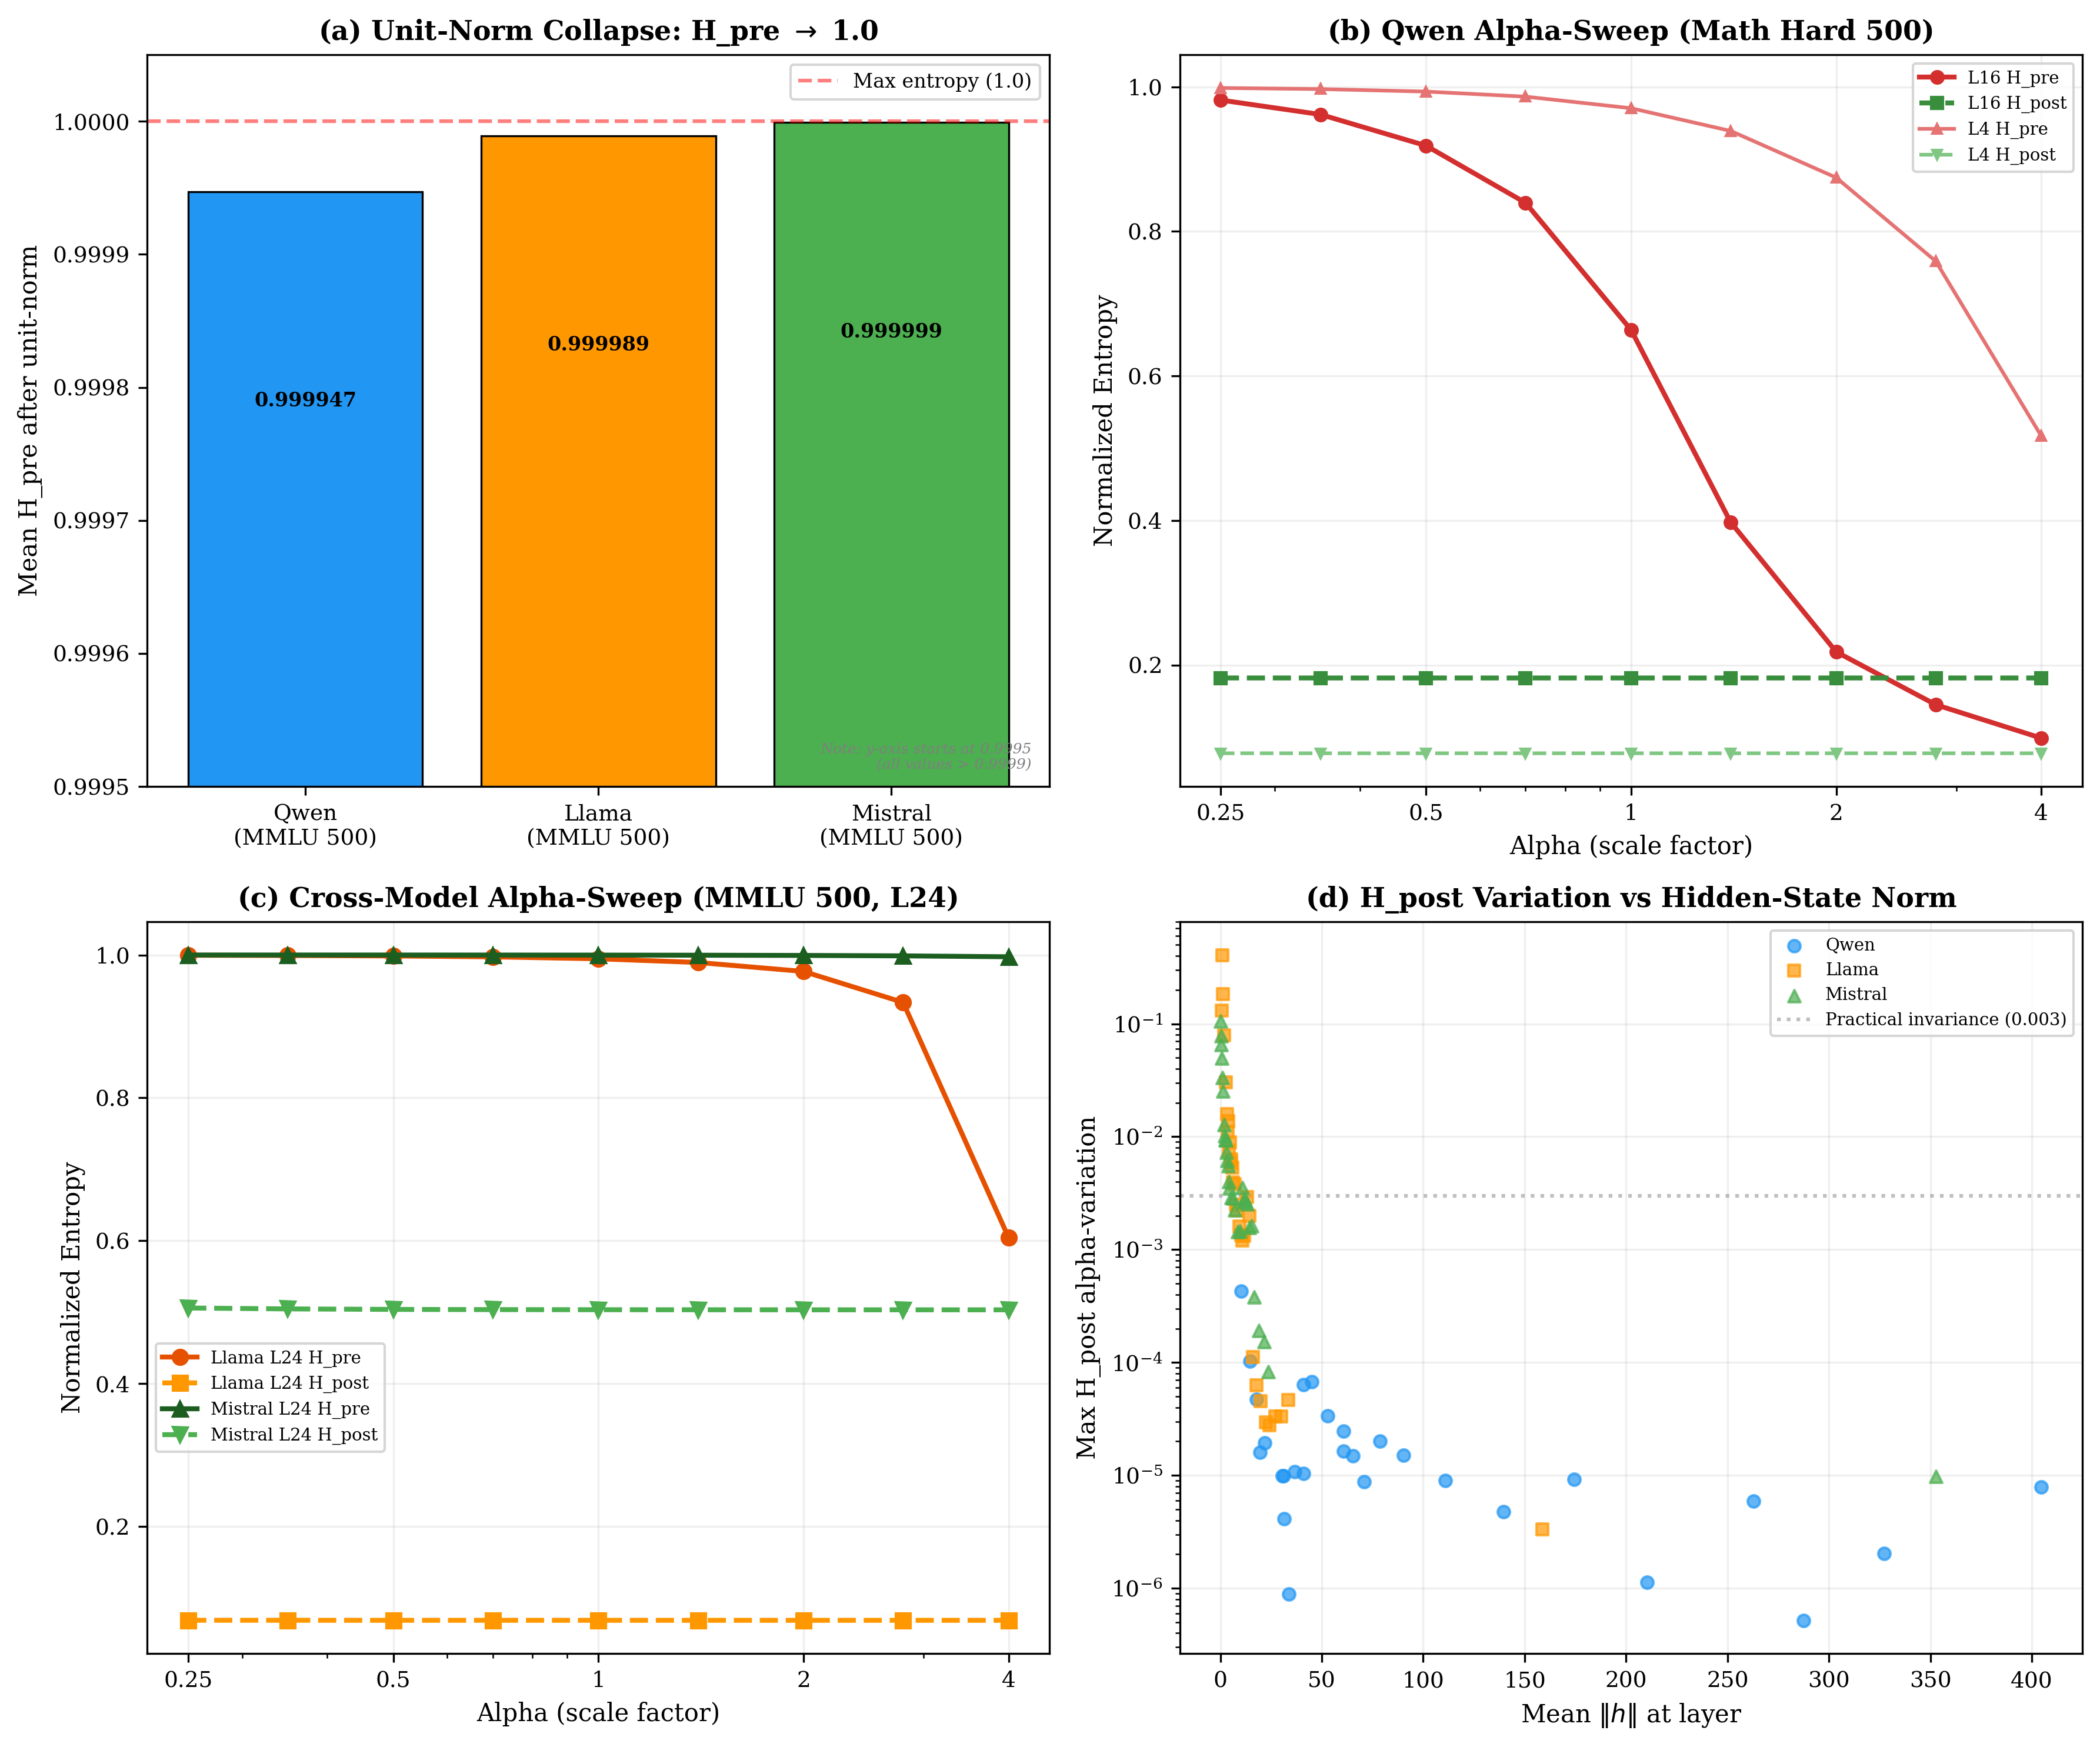
\includegraphics[width=\textwidth]{fig2.png}
\caption{Scale intervention results. (a)~Unit-norm removal collapses $\Hpre$ toward maximal entropy ($\sim$1.0) while $\Hpost$ changes by less than 0.003. (b)~Alpha-sweep on Qwen: $\Hpre$ responds strongly to scale manipulation; $\Hpost$ remains invariant to four decimal places. (c)~Cross-model alpha-sweep at L24 (Llama and Mistral). (d)~$\Hpost$ variation vs.\ hidden-state norm.}
\label{fig:scale_intervention}
\end{figure*}

On Qwen, $\Hpre$ spans the range 0.10--0.98 under alpha-sweep at L16, while $\Hpost$ shows zero variation to four decimal places. The top-1 decoded token is invariant under positive scaling---$\arg\max(\alpha Wh) = \arg\max(Wh)$ for any $\alpha > 0$---so prior findings that normalization does not affect top-token interpretations \cite{geva2022transformer} are fully consistent with our results. The distinction is that entropy depends on the full probability distribution, not just its mode. This establishes $\Hpre$ as scale-sensitive and $\Hpost$ as effectively scale-invariant on this model, while confirming that top-token and entropy-based analyses address different properties of intermediate representations.

\subsection{Cross-Family Verification}

To verify that these findings are not Qwen-specific, we repeat the intervention on all three models using identical conditions (Table~\ref{tab:crossmodel}): 500 MMLU samples, Step~0, seed~=~42.

\begin{table}[!h]
\centering
\caption{Cross-model scale intervention summary (MMLU 500, Step~0, seed~=~42). ``\% orig.\ $\Hpre{>}0.99$'' reports layers where unmodified $\Hpre$ already exceeds 0.99 (ceiling effect), distinct from the unit-norm row where all models converge to ${\sim}$1.0 by construction.}
\label{tab:crossmodel}
\footnotesize
\setlength{\tabcolsep}{3pt}
\begin{tabular}{l ccc}
\toprule
 & \textbf{Qwen} & \textbf{Llama} & \textbf{Mistral} \\
\midrule
Layers & 28 & 32 & 32 \\
$\Hpre$ unit-norm mean & 0.999947 & 0.999989 & 0.999999 \\
Max $\Delta\Hpost$ ($\alpha$) & 0.000428 & 0.406987 & 0.105264 \\
Worst layer & L0 & L1 & L0 \\
h\_norm at worst & 10.21 & 0.89 & 0.25 \\
\% orig.\ $\Hpre{>}0.99$ & 0\% & 66\% & 91\% \\
\bottomrule
\end{tabular}
\end{table}

Across all three model families tested, unit-normalization collapses $\Hpre$ toward maximal entropy (mean~$>$~0.9999), confirming that $\Hpre$ is scale-sensitive in these RMSNorm-based settings (Fig.~\ref{fig:scale_intervention}).

$\Hpost$ is largely scale-invariant in middle and late layers: at L16, alpha-sweep variation is 0.0022 (Llama) and 0.0028 (Mistral). At L24, Llama achieves near-exact invariance ($\Hpost$ = 0.0689--0.0690 across all alpha values).

\subsection{Low-Norm Early-Layer Exception}
\label{sec:epsilon}

$\Hpost$ alpha-invariance breaks down in early layers: Llama L1 shows variation of 0.407, Mistral L0 shows 0.105, while Qwen L0 shows only 0.0004. Two factors contribute to these deviations:

\textbf{Hidden-state norm (primary factor).} The deviations correlate with hidden-state norm: Mistral L0 has mean h\_norm~=~0.25, Llama L1 has 0.89, while Qwen L0 has 10.21 (all under MMLU 500, Step~0). When the layer RMS is very small, the epsilon term in RMSNorm becomes non-negligible under alpha-scaling, breaking exact invariance.

\textbf{Epsilon value (secondary factor).} Llama and Mistral use $\epsilon = 10^{-5}$ (10$\times$ larger than Qwen's $10^{-6}$). At a given hidden-state norm, a larger epsilon increases the ratio $\epsilon/\text{mean}(h^2)$, amplifying the deviation. However, counterfactual analysis shows that even with $\epsilon = 10^{-6}$, Mistral L0 would still show substantial deviation because h\_norm~=~0.25 is so small that $\text{mean}(h^2) = \text{h\_norm}^2/d$ is itself comparable to the effective epsilon term: at $\alpha = 0.25$, $(\epsilon/\alpha^2)/\text{mean}(h^2) = 1.05$, meaning the epsilon contribution in the denominator is as large as the signal.

We therefore treat $\Hpost$ as largely scale-invariant in the operating regime of middle and late layers, with explicit low-norm early-layer deviations driven primarily by small hidden-state norms and secondarily by epsilon magnitude.

\subsection{Saturation-Limited Observability}
\label{sec:saturation}

While unit-norm removal establishes that scale sensitivity \textit{exists} structurally, the alpha-sweep reveals that its \textit{observable magnitude} varies dramatically across models:

In Llama and Mistral, $\Hpre$ is already near maximal entropy ($\sim$1.0) in early-to-middle layers because hidden-state norms are small (Mistral L0: 0.25 vs.\ Qwen L0: 10.21), as shown in Fig.~\ref{fig:saturation} (Appendix~\ref{app:decoder_controls}; Qwen dynamic range 0.924 vs.\ Llama 0.008, Mistral 0.0005). This ceiling effect compresses the observable alpha-sweep response, making scale sensitivity practically invisible in intermediate layers despite being structurally present.

\begin{figure*}[!t]
\centering
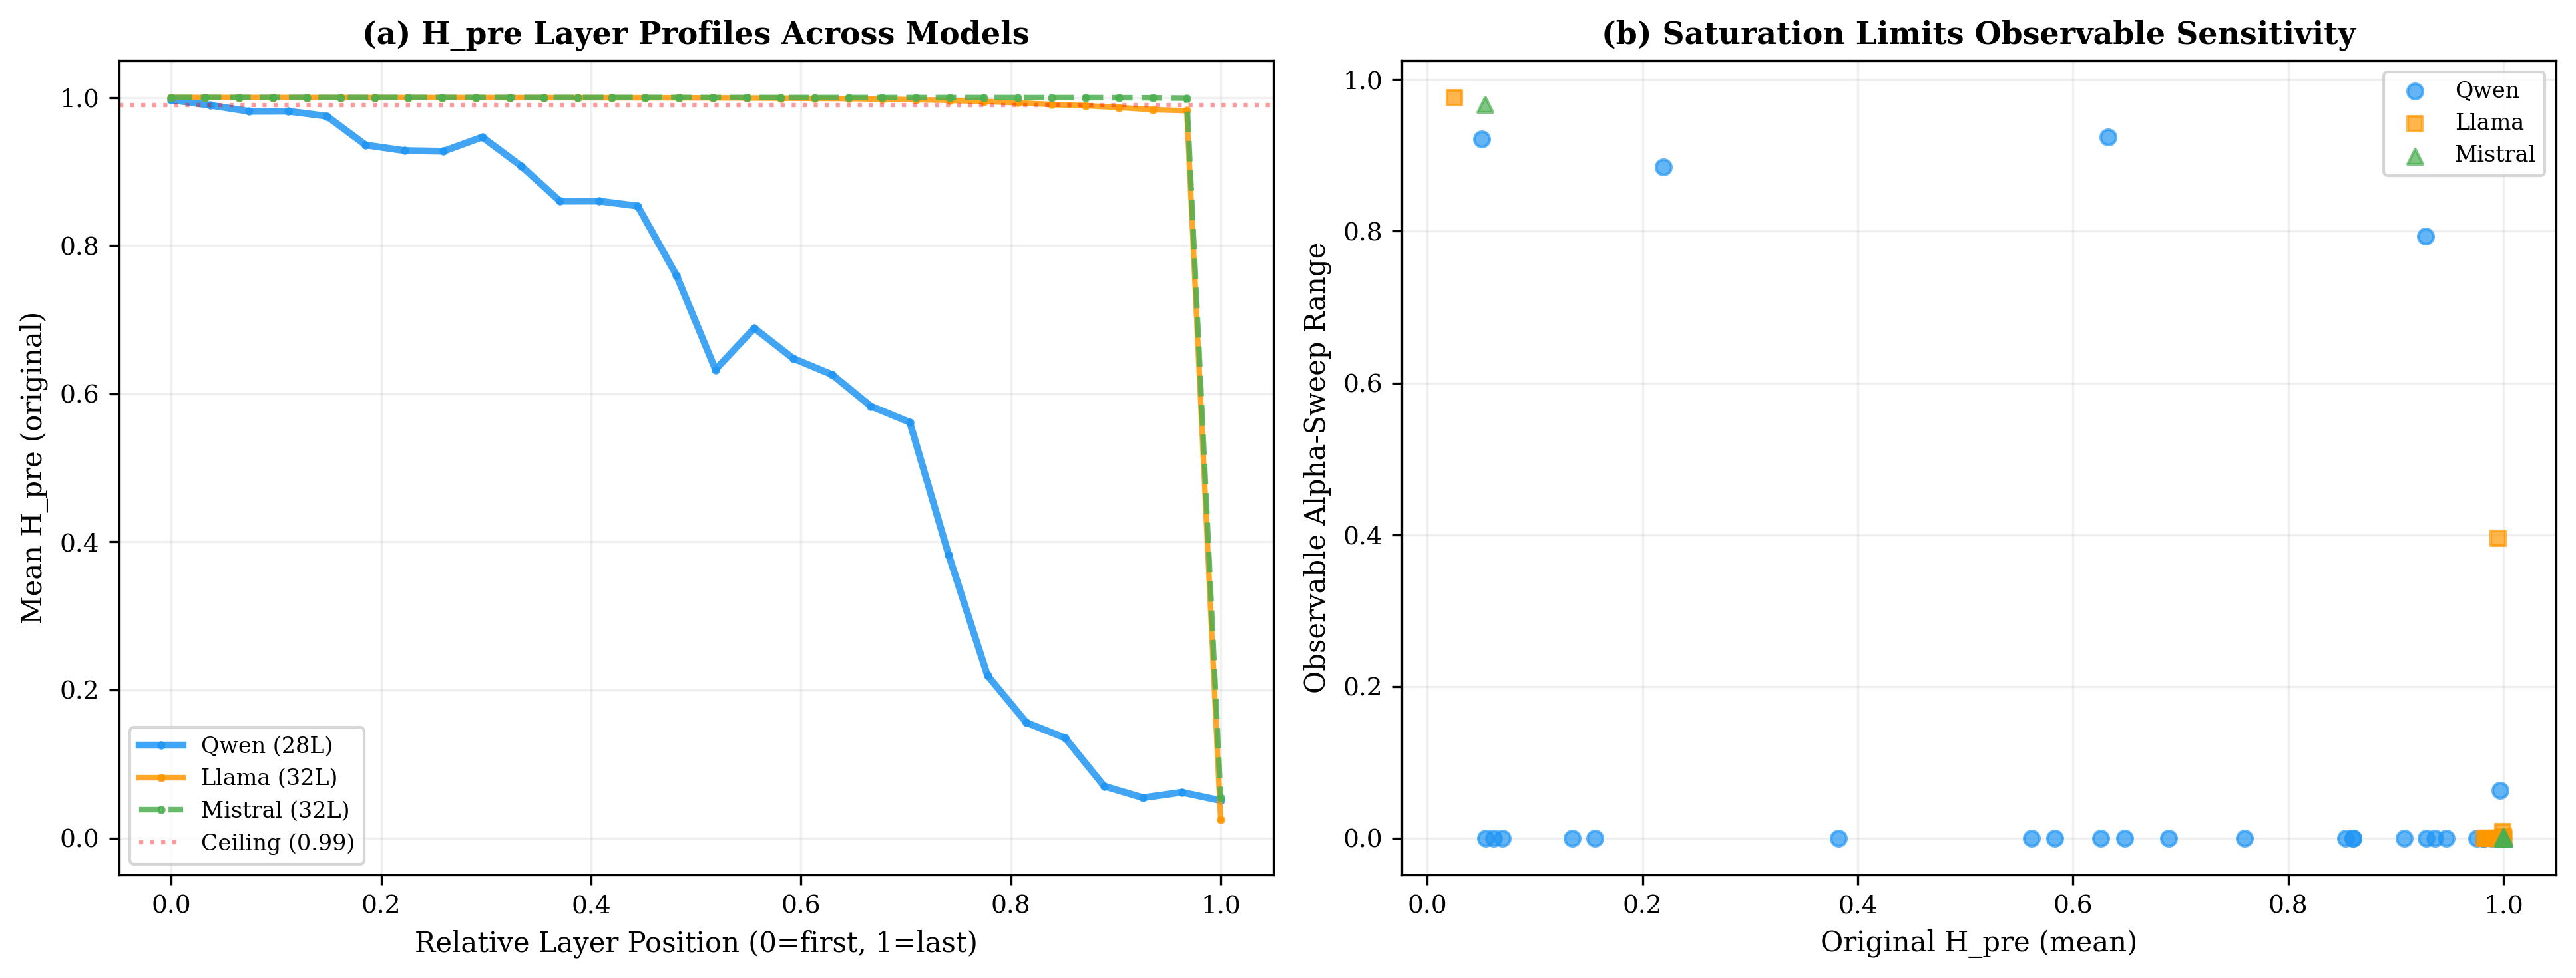
\includegraphics[width=\textwidth]{fig3.png}
\caption{Layerwise profile and saturation. (a)~$\Hpre$ layer profiles across models: Qwen shows wide dynamic range (0.02--1.0), while Llama and Mistral are near ceiling ($\sim$1.0) in early-to-middle layers. (b)~Observable alpha-sweep range vs.\ original $\Hpre$: high $\Hpre$ layers have negligible observable range (saturation effect).}
\label{fig:saturation}
\end{figure*}

Norm-binned control results corroborate this (Appendix~\ref{app:normbinned}): when $\Hpre$ is controlled for logit\_std, Mistral retains 100.1\% of its AUROC---not because $\Hpre$ is scale-invariant, but because $\Hpre$ is already at ceiling and carries little additional information beyond scale. In contrast, Mistral's $\Hpre$ retention after controlling for h\_norm is 85.2\% (Appendix~\ref{app:normbinned}).

$\Hpre$ is scale-sensitive, but the observable magnitude of this sensitivity is saturation-limited and therefore model- and layer-dependent.

\subsection{Correlational Radial/Angular Analysis}
\label{sec:radial_angular}

The intervention results above establish functional scale sensitivity: changing hidden-state norm changes $\Hpre$ in all three model families. This does not imply that norm explains most cross-sample variation in $\Hpre$ on a given dataset. To separate these notions, we analyzed how much of the cross-sample variation in $\Hpre$ is accounted for by radial magnitude ($\|h_l\|$) versus angular direction. For each layer, we compute the linear $R^2$ and Spearman $|\rho|$ between $\Hpre$ and $\|h_l\|$ across samples under both sampled and greedy protocols.

Llama and Mistral show strong norm coupling ($R^2 > 0.82$, mean across layers), meaning most cross-sample $\Hpre$ variation covaries with hidden-state magnitude. Qwen shows much weaker coupling ($R^2 \approx 0.15$), indicating that direction---not magnitude---drives most of the cross-sample $\Hpre$ variation in that model. This pattern is stable across protocols (sampled vs.\ greedy). Full decomposition details including per-protocol CIs are provided in the repository.

This does not contradict Sections~\ref{sec:qwen_case}--\ref{sec:saturation}: norm remains causally important under intervention (unit-norm removal collapses Qwen $\Hpre$ just as completely as for Llama/Mistral), but the degree to which \textit{naturally occurring} $\Hpre$ variation is norm-dominated is model-dependent. At the profile level, however, predictive redundancy persists across all three models: scale-correlated profiles match or exceed $\Hpre$ profiles for correctness discrimination regardless of the underlying radial/angular composition (Section~\ref{sec:profile_redundancy}). The main predictive claim of C2 is therefore not that norm explains most variance of $\Hpre$ in every model, but that scale-correlated profiles already capture most of $\Hpre$'s correctness-discriminative content. Full layer-by-layer decomposition details are in Appendix~\ref{app:radial}.


%===============================================================================
\section{Predictive Utility of Internal Signals}
\label{sec:predictive}

Section~\ref{sec:what} established that $\Hpre$ is scale-sensitive and that this sensitivity has large empirical magnitude. We now evaluate which internal signals best discriminate correct from incorrect responses and test whether $\Hpre$ carries information beyond what simple scale proxies already capture.

\subsection{Internal Layers Provide Additional Discrimination Beyond Final-Output Entropy}

Table~\ref{tab:baseline} presents one representative held-out split (70/30, seed~=~42) for four primary evaluation conditions under the generation-average protocol (post-generation diagnostics). The main empirical finding is that, under this sampled-generation protocol, $\Hpre$ often does not outperform scale-correlated baselines (logit\_std, h\_norm). This ordering is robust within the sampled protocol: in a 20-split repeated analysis (Section~\ref{sec:robustness}), logit\_std outperforms $\Hpre$ in 79/80 condition-split combinations (100\% in three conditions, 95\% in Qwen MMLU). Under greedy decoding on the same items, the single-layer ordering logit\_std~$>$~$\Hpre$ is preserved on all three models (Section~\ref{sec:greedy}), though greedy repeated-split analysis shows reduced sign stability (Section~\ref{sec:robustness}), indicating that single-layer comparisons are sensitive to decoding protocol.

\begin{table}[!h]
\centering
\caption{Held-out test AUROC---selected scalar baselines (H = Hard, M = MMLU). Bold indicates highest AUROC in each column. [Protocol: sampled generation, generation-average, 70/30 split seed=42]}
\label{tab:baseline}
\footnotesize
\setlength{\tabcolsep}{3pt}
\begin{tabular}{l cccc}
\toprule
Method & Qwen H & Qwen M & Llama M & Mistral M \\
\midrule
logit\_std & 0.8086 & \textbf{0.6674} & \textbf{0.6522} & \textbf{0.7315} \\
h\_norm & \textbf{0.8256} & 0.5740 & 0.5763 & 0.6983 \\
$\Hpre$ & 0.7672 & 0.6367 & 0.6021 & 0.6737 \\
$\Hpost$ & 0.6613 & 0.6376 & 0.5796 & 0.5850 \\
Output entropy & 0.6316 & 0.5775 & 0.5354 & 0.5070 \\
\bottomrule
\end{tabular}
\end{table}

\begin{figure*}[!t]
\centering
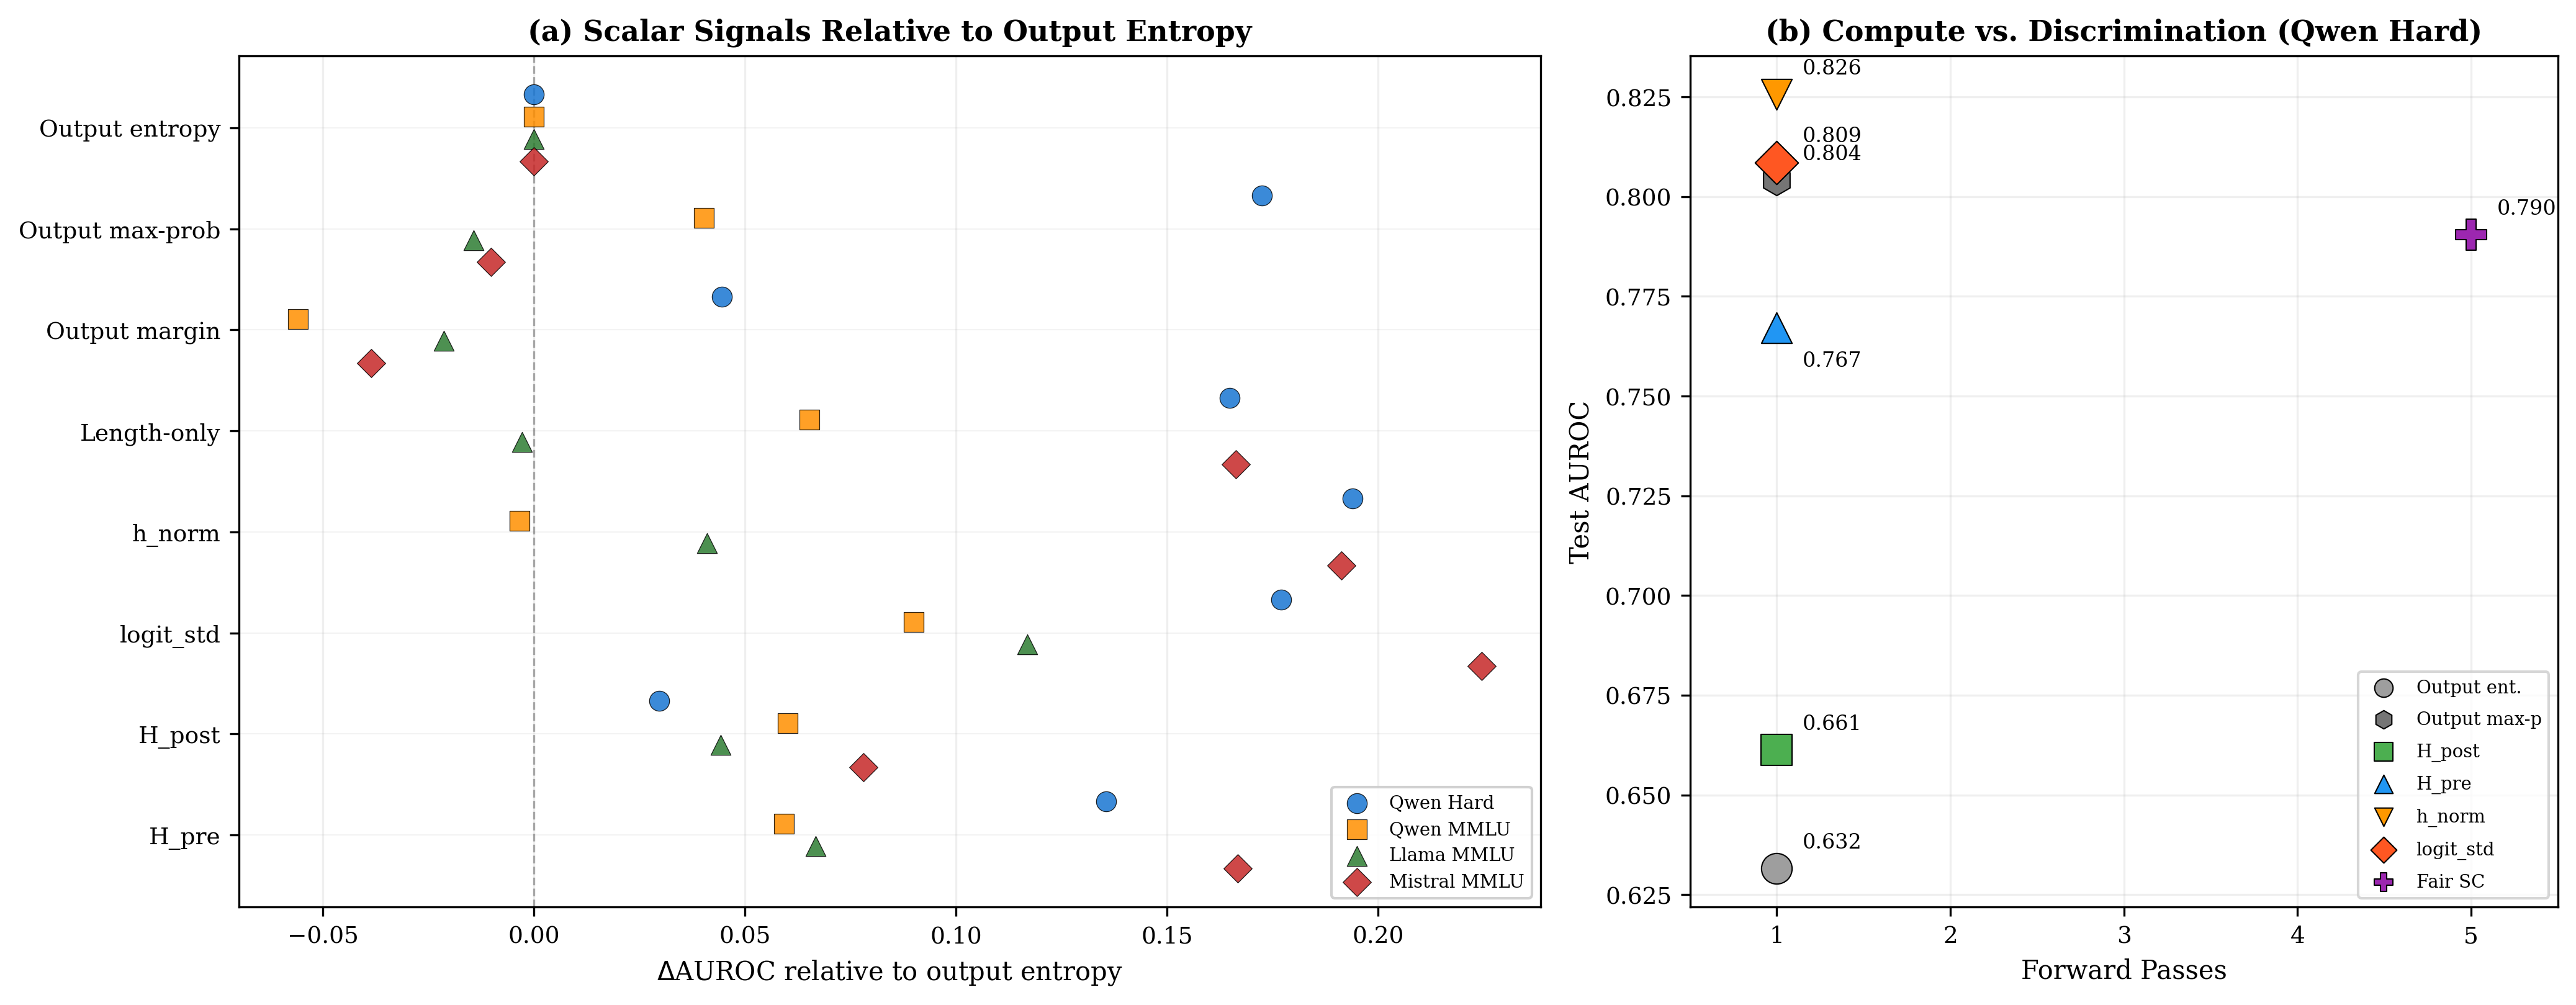
\includegraphics[width=\textwidth]{fig4.png}
\caption{Baseline comparison. (a)~$\Delta$AUROC of scalar signals relative to output entropy across four primary conditions. logit\_std outperforms single-layer $\Hpre$ in all four conditions; h\_norm does so in two of four. (b)~Compute vs.\ discrimination tradeoff on Qwen Hard: logit\_std (1 forward pass) achieves higher AUROC than matched self-consistency (5 passes).}
\label{fig:baseline}
\end{figure*}

The baseline comparison (Fig.~\ref{fig:baseline}) reveals two patterns central to the measurement non-equivalence:

\begin{enumerate}
\item \textbf{Among single-layer scalars, scale-correlated baselines outperform $\Hpre$}: logit\_std outperforms single-layer $\Hpre$ in all four sampled-generation conditions and in all three models under greedy decoding (Section~\ref{sec:greedy}). This ordering is robust at the single-split level, though greedy repeated-split analysis shows reduced sign/layer stability (Section~\ref{sec:robustness}; Appendix~\ref{app:greedy}). Multi-layer $\Hpre$ profiles outperform single-layer scale proxies, suggesting that the full entropy trajectory carries information beyond a single scalar.

\item \textbf{Internal layers outperform final-output entropy}: In all four sampled-generation conditions, the best internal-layer signal exceeds output entropy by +0.09 to +0.22 AUROC. Under greedy decoding, logit\_std matches or exceeds output entropy on all three models (0.683 vs.\ 0.682 on Qwen, 0.700 vs.\ 0.462 on Llama, 0.727 vs.\ 0.472 on Mistral), preserving this advantage. Multi-layer profiles further outperform output entropy under both protocols (Section~\ref{sec:greedy}). Additional output-level baselines (max-prob, margin, length-only) are reported in Appendix~\ref{app:additional}.
\end{enumerate}

Multi-layer profiles consistently outperform the best single-layer scalar by +0.01 to +0.06 AUROC (detailed profile comparisons provided in the repository). Among profiles, h\_norm profile is strongest in 3/4 conditions, reflecting scale as an important driver of discrimination.

\FloatBarrier
\subsection{For Single-Layer Scalars, $\Hpre$ Shows Limited Incremental Utility Over Scale Proxies}
\label{sec:profile_redundancy}

The results in Table~\ref{tab:baseline} show that logit\_std outperforms $\Hpre$ in all four conditions. If $\Hpre$'s correctness-discriminative content is largely carried by scale-correlated variation, then adding $\Hpre$ to logit\_std should yield little incremental information, because both features respond to overlapping aspects of hidden-state magnitude. We test this prediction directly across all four primary conditions. We fit logistic regression models with and without $\Hpre$ on the calibration set and evaluate on the held-out test set (Table~\ref{tab:incremental}).

\begin{table}[!h]
\centering
\caption{Incremental utility of $\Hpre$ over scale proxies (held-out test AUROC; H = Hard, M = MMLU). [Protocol: sampled, gen-avg, 70/30 split]}
\label{tab:incremental}
\footnotesize
\setlength{\tabcolsep}{1.5pt}
\begin{tabular}{l cccc}
\toprule
Features & Qwen H & Qwen M & Llama M & Mistral M \\
\midrule
logit\_std only & 0.8086 & 0.6674 & 0.6522 & 0.7315 \\
$\Hpre$ only & 0.7672 & 0.6367 & 0.6021 & 0.6737 \\
logit\_std + $\Hpre$ & 0.8284 & 0.6705 & 0.6522 & 0.7366 \\
logit\_std+h\_norm+len & 0.8120 & 0.6466 & 0.6589 & 0.7267 \\
+$\Hpre$ & 0.8143 & 0.6427 & 0.6714 & 0.7430 \\
\midrule
$\Delta$(+$\Hpre$) & +0.020 & +0.003 & +0.000 & +0.005 \\
95\% CI & [{-}.014,{+}.057] & [{-}.003,{+}.009] & [{-}.006,{+}.005] & [{-}.007,{+}.017] \\
$\Delta$(full+$\Hpre$) & +0.002 & $-$0.004 & +0.012 & +0.016 \\
95\% CI & [{-}.022,{+}.027] & [{-}.012,{+}.003] & [{-}.002,{+}.027] & [{+}.005,{+}.029] \\
\bottomrule
\end{tabular}
\end{table}

Under the sampled-generation protocol, none of the four conditions yields a 95\% bootstrap CI excluding zero when adding $\Hpre$ to logit\_std (paired bootstrap, 1000 resamples). This result holds across all three model families, including Llama and Mistral where $\Hpre$ dynamic range is more limited due to saturation (Section~\ref{sec:saturation}). Under greedy decoding, the zero-incremental-utility finding is confirmed across all three models (Section~\ref{sec:greedy}), with CIs including zero in every case. Profile-level redundancy likewise holds under both protocols. Scale-correlated variation therefore captures most of $\Hpre$'s correctness-discriminative content in the tested settings: logit\_std---a more direct measure of that variation---leaves little incremental utility for $\Hpre$. One exception: under the full feature set (logit\_std + h\_norm + length), adding $\Hpre$ yields a nominal-level delta on Mistral MMLU (+0.016, CI [+0.005, +0.029]). Across the eight primary tests (4~conditions $\times$ 2~feature sets), this single CI-excluding-zero result does not survive Bonferroni correction ($\alpha/8 = 0.00625$). We note this as a potential exception rather than a robust counterexample; it reappears in the exceptions inventory in Section~\ref{sec:implications}.

This redundancy extends to multi-layer profiles. When using the full layer profile (all layers as features) with logistic regression and 5-fold cross-validation, the scale-baseline profile (logit\_std + h\_norm) achieves AUROC 0.709--0.844 across the four conditions. Adding the full $\Hpre$ profile yields deltas of $-$0.001 to +0.001---effectively zero incremental utility even at the profile level. Adding $\Hpost$ profiles yields similarly negligible deltas ($-$0.001 to +0.006). Under greedy decoding, profile-level redundancy is confirmed: adding $\Hpre$ to the scale profile yields deltas of $-$0.007 to +0.000 across all three models (Section~\ref{sec:greedy}, Table~\ref{tab:greedy}). Scale redundancy is therefore not an artifact of single-layer evaluation or decoding protocol: even when the classifier has access to the entire layerwise entropy trajectory, entropy profiles add little discriminative information beyond what scale profiles already capture.

\textbf{Length confound control.} Since incorrect responses tend to be longer (mean token count: correct 245--302 vs.\ incorrect 258--358 across models), generation length could confound entropy-based discrimination. We control for this via three methods: (i) residualizing entropy against length via linear regression, (ii) computing within-length-tertile AUROC, and (iii) comparing length-only vs.\ length+entropy logistic regression. $\Hpost$ retains 95--103\% of its original AUROC after length residualization across all conditions, confirming that its signal is not a length artifact. $\Hpre$ retains 77--104\%, and logit\_std retains 71--97\%---both showing partial confounding with length, as expected for scale-sensitive metrics that co-vary with generation effort. Adding entropy to a length-only baseline yields incremental AUROC of +0.001 to +0.047 across conditions, with $\Hpost$ and h\_norm showing the largest increments. Full results in Appendix~\ref{app:length}.

\FloatBarrier
\subsection{Robustness of the Main Protocol}
\label{sec:robustness}

The headline results in Tables~\ref{tab:baseline}--\ref{tab:incremental} are based on a single 70/30 calibration/test split (seed~=~42). To assess partition sensitivity, we conduct a 20-split repeated stratified analysis (seeds 0--19), applying the same protocol: best layer and sign selected on each calibration fold, evaluated on the corresponding test fold. Key findings from the repeated-split analysis (full details in Appendix~\ref{app:repeated}):

\textbf{Ordering stability.} The ordering logit\_std~$>$~$\Hpre$ is maintained in 79/80 condition-split combinations: 20/20 on Qwen Hard, Llama MMLU, and Mistral MMLU; 19/20 on Qwen MMLU. Mean AUROC across splits: logit\_std = 0.642--0.772, $\Hpre$ = 0.605--0.736. On Qwen MMLU, $\Hpost$ (0.661~$\pm$~0.023) outperforms logit\_std (0.642~$\pm$~0.031) in the majority of splits.

\textbf{Sign stability (sampled generation).} $\Hpre$ sign (lower = correct) is fully stable under sampled generation: 80/80 condition-split combinations show sign~=~$-1$. Under greedy decoding, this stability degrades (10--13/20; Section~\ref{sec:greedy}, Appendix~\ref{app:greedy}). $\Hpost$ sign shows cross-family reversal: sign~=~+1 in 15/20 Llama splits vs.\ $-1$ on Qwen and Mistral (20/20 each), confirming that sign calibration on a held-out set is necessary. Additionally, h\_norm on Qwen MMLU shows sign~=~$-1$ in only 10/20 splits (effectively 50/50), making it the only metric-condition pair with no dominant sign direction.

\textbf{Layer variability.} Some metrics show high layer stability (h\_norm on Qwen Hard: L18 in 20/20 splits; $\Hpost$ on Qwen MMLU: L27 in 20/20), while others show substantial variability (logit\_std on Qwen Hard: L4 in 9/20, L16 in 6/20; $\Hpre$ on Qwen MMLU: L18 in 7/20, L12 in 7/20). AUROC standard deviations range from 0.022 to 0.057 across conditions.

\textbf{Implication.} The qualitative conclusions---scale proxies matching or exceeding $\Hpre$, internal layers providing additional discrimination beyond output-only entropy---are robust to partition choice under sampled generation. Exact layer selections and AUROC values should be treated as representative rather than definitive. Section~\ref{sec:greedy} tests whether these findings also hold under deterministic (greedy) decoding.

\textbf{Multi-seed generation robustness.} The repeated-split analysis above varies the calibration/test partition but holds the generated text fixed. To test whether conclusions are stable across different generation runs, we re-run the full Qwen MMLU pipeline with two additional generation seeds (123 and 456), using the same 1000 questions (data selection seed fixed at 42) and the same protocol (temperature~=~0.3, generation-average features, 70/30 split). Both seeds produce 74.4\% accuracy (vs.\ 74.9\% at seed~42). Across the two reruns, profile-level AUROC ordering is preserved: logit\_std profile AUROC~=~0.795/0.771 (seeds 123/456), $\Hpre$ profile~=~0.786/0.749, $\Hpost$ profile~=~0.786/0.781, and h\_norm profile~=~0.773/0.783. The ordering logit\_std~$\geq$~$\Hpre$ holds in both seeds, and $\Hpre$ incremental utility over logit\_std remains near zero (delta~=~$-$0.003 and $-$0.011). Best-layer agreement is 3/4 primary metrics across seeds; the sole exception is $\Hpre$ (L12 vs.\ L16), while $\Hpost$ remains L27 in both seeds. Across all eight scalar metrics, agreement is 7/8. Full details appear in Appendix~\ref{app:multiseed}.

\textbf{Task extension.} A preliminary extension to TruthfulQA mc1 \cite{lin2022truthfulqa} (817 items, Qwen; Appendix~\ref{app:truthfulqa}) shows a similar profile-level ordering (h\_norm 0.756 $>$ logit\_std 0.744 $>$ $\Hpre$ 0.742 $>$ $\Hpost$ 0.725), but $\Hpre$ incremental utility over logit\_std is a small positive (+0.016) rather than the near-zero or negative values observed on MMLU. This pattern suggests weaker scale redundancy on factual-knowledge benchmarks with variable choice counts. This is a single-model, single-split observation without confidence intervals.

\FloatBarrier
\subsection{Greedy Decoding: What is Robust and What is Protocol-Sensitive}
\label{sec:greedy}

The main evaluation protocol uses stochastic generation (temperature~=~0.3, \texttt{do\_sample~=~True}), which introduces two sources of non-determinism: (1) different generated text across runs, and (2) generation-average features that depend on the specific tokens produced. To test whether our findings are artifacts of stochastic evaluation, we re-evaluate on the same 1000 MMLU items using greedy decoding (\texttt{do\_sample~=~False}), which produces deterministic outputs and features.

\textbf{Greedy protocol.} Same 0-shot chat template, same \texttt{max\_new\_tokens~=~1024}, same per-layer feature computation (generation-average), same 70/30 held-out split (seed~=~42). Only the decoding strategy differs: greedy (\texttt{do\_sample~=~False}) instead of sampled (temperature~=~0.3).

\textbf{Agreement between sampled and greedy labels.}

Agreement rates of 82--90\% (kappa 0.60--0.73) indicate substantial overlap with moderate divergence (detailed agreement table provided in the repository), confirming that switching to greedy decoding changes both the correctness labels and the feature distributions.

\textbf{Single-layer results under greedy (Table~\ref{tab:greedy}).}

\begin{table}[!h]
\centering
\caption{Greedy decoding results (same 1000 MMLU items as Table~\ref{tab:baseline}). [Protocol: greedy, gen-avg]}
\label{tab:greedy}
\footnotesize
\setlength{\tabcolsep}{4pt}
\begin{tabular}{l ccc}
\toprule
\multicolumn{4}{c}{\textit{Panel A. Single-layer held-out AUROC (layer)}} \\
\midrule
Method & Qwen & Llama & Mistral \\
\midrule
logit\_std & \textbf{0.683} (L12) & \textbf{0.700} (L13) & \textbf{0.727} (L14) \\
h\_norm & \textbf{0.683} (L18) & 0.632 (L0) & 0.698 (L14) \\
$\Hpre$ & 0.604 (L18) & 0.658 (L0) & 0.688 (L30) \\
$\Hpost$ & 0.682 (L27) & 0.646 (L10) & 0.500 (L24) \\
Output entropy & 0.682 & 0.462 & 0.472 \\
\midrule
\multicolumn{4}{c}{\textit{Panel B. Incremental utility}} \\
\midrule
logit\_std only & 0.683 & 0.700 & 0.727 \\
logit\_std + $\Hpre$ & 0.673 & 0.697 & 0.728 \\
$\Delta$ [95\% CI] & $-$0.010 & $-$0.003 & +0.000 \\
 & [{-}.030,{+}.008] & [{-}.007,{+}.001] & [{-}.001,{+}.002] \\
\midrule
\multicolumn{4}{c}{\textit{Panel C. Profile AUROC (5-fold CV, LR)}} \\
\midrule
$\Hpre$ profile & 0.744 & 0.668 & 0.711 \\
scale (combined) & \textbf{0.765} & \textbf{0.676} & \textbf{0.764} \\
scale + $\Hpre$ & 0.758 & 0.673 & \textbf{0.764} \\
$\Delta$ & $-$0.007 & $-$0.004 & +0.000 \\
\bottomrule
\end{tabular}
\end{table}

Two findings emerge from Panel~A. First, logit\_std outperforms $\Hpre$ on all three models under greedy decoding (by +0.079 on Qwen, +0.042 on Llama, +0.039 on Mistral), matching the sampled-generation ordering (Table~\ref{tab:baseline}). Second, logit\_std matches or exceeds output entropy on all three models (Qwen: 0.683 vs.\ 0.682, essentially tied; Llama and Mistral: clear margins), so the ``internal layers match or exceed output'' pattern is preserved under greedy for scale-correlated baselines.

Under greedy decoding, $\Hpre$ provides no incremental utility over logit\_std on any of the three models (all CIs include zero, Panel~B), confirming the sampled-generation finding. At the profile level, scale profiles match or outperform $\Hpre$ profiles in all three models under greedy decoding (Panel~C). The qualitative landscape distinction is also preserved: under greedy, $\Hpre$ remains comparatively flat across many layers while $\Hpost$ is more sharply concentrated. This $\Hpost$-peaked / $\Hpre$-flat contrast is the most robust landscape pattern across protocols (Appendix~\ref{app:greedy}).

\textbf{Summary.} Profile-level scale redundancy (3/3 models), landscape contrast ($\Hpost$ peaked / $\Hpre$ flat), internal-layer advantage over output entropy, and single-layer incremental CI containing zero all hold under both sampled and greedy protocols. Classifier sensitivity (LR $>$ $k$-NN) was tested under sampled generation only. Two aspects deserve emphasis. First, although sampled and greedy labels agree substantially (82--90\%, kappa 0.60--0.73), single-layer repeated-split analysis (Appendix~\ref{app:greedy}) confirms that sign stability degrades to 10--13/20 (vs.\ 20/20 under sampled generation) and layer selections are weakly concentrated---the single-split orderings above should therefore be interpreted cautiously. Second, the profile-vs-single-layer gap remains large under greedy (single-layer $\Hpre$ AUROCs are 0.604--0.688 while profile AUROCs are 0.668--0.764), supporting the recommendation to use multi-layer profiles rather than single-layer scalars.


%===============================================================================
\FloatBarrier
\section{Where and When the Signal Appears}
\label{sec:where}

This section provides secondary characterization of where and when the decoded-entropy signal appears---token position, layer variability, and sign direction. These are robustness and contextual analyses that complement the primary evidence in Sections~\ref{sec:what}--\ref{sec:predictive}.

\subsection{Token Position}
\label{sec:token_position}

We compare three extraction positions across all three models on MMLU (1000 samples each, same items as the baseline evaluation; Appendix~\ref{app:token}). Full-generation average yields the highest AUROC for most metrics (10/12 model-metric combinations). The exceptions are $\Hpost$ on Llama and Mistral, where Step~1 (first generated token) is optimal, indicating that $\Hpost$ captures directional information that is strongest at the generation onset. Step~0 (prompt-last, pre-generation) carries above-chance signal in all conditions (AUROC 0.54--0.68), indicating that pre-generation discrimination is possible. Different metrics favor different positions, and these preferences are not consistent across models.

\subsection{No Universal Optimal Layer Under Our Protocol}

Under our held-out protocol (single 70/30 split, seed~=~42), the best-performing layer varies substantially across conditions and model families (exact layer/sign selections provided in the repository): e.g., Qwen $\Hpre$ best = L17 vs.\ Llama $\Hpre$ best = L0. No fixed optimal layer emerges for correctness discrimination. The best layer depends on the metric, model family, and task. These selections are based on a single split; Appendix~\ref{app:repeated} quantifies their partition sensitivity using 20 repeated stratified splits (see also Section~\ref{sec:sign_reversal}).

Optimal-layer conclusions are sensitive to both metric choice and evaluation protocol (Fig.~\ref{fig:perlayer_d}): e.g., Mistral $\Hpre$ best = L0 under full-sample Cohen's $d$ vs.\ L30 under held-out AUROC.

\subsection{Cross-Family Sign Reversal}
\label{sec:sign_reversal}

Repeated-split analysis (20 independent 70/30 splits, seeds 0--19) under sampled generation reveals that $\Hpre$ sign is fully stable: lower $\Hpre$ is associated with correct responses (sign~=~$-$) across all four conditions and all 20 splits (20/20). However, $\Hpost$ exhibits cross-family sign instability: on Llama MMLU, $\Hpost$ sign is $+$ in 15/20 splits (higher $\Hpost$ = correct), reversing the $-$ sign observed in all Qwen and Mistral conditions. This precludes a fixed-sign heuristic for $\Hpost$ and necessitates sign calibration on a held-out set. Under sampled generation, the sign reversal is specific to $\Hpost$, not $\Hpre$. However, under greedy decoding, $\Hpre$ sign stability also degrades (Section~\ref{sec:greedy}), indicating that sign stability depends on the decoding protocol as well as the metric.

\subsection{Multi-Layer Profiles}

Using logistic regression over all-layer features, the h\_norm profile outperforms the best single-layer scalar in all four conditions, whereas the $\Hpre$ profile does so in three of four. The $\Hpre$ profile gain over its own best single-layer ranges from +0.022 to +0.099 across conditions, further supporting the role of scale in discrimination.

\begin{figure*}[!t]
\centering
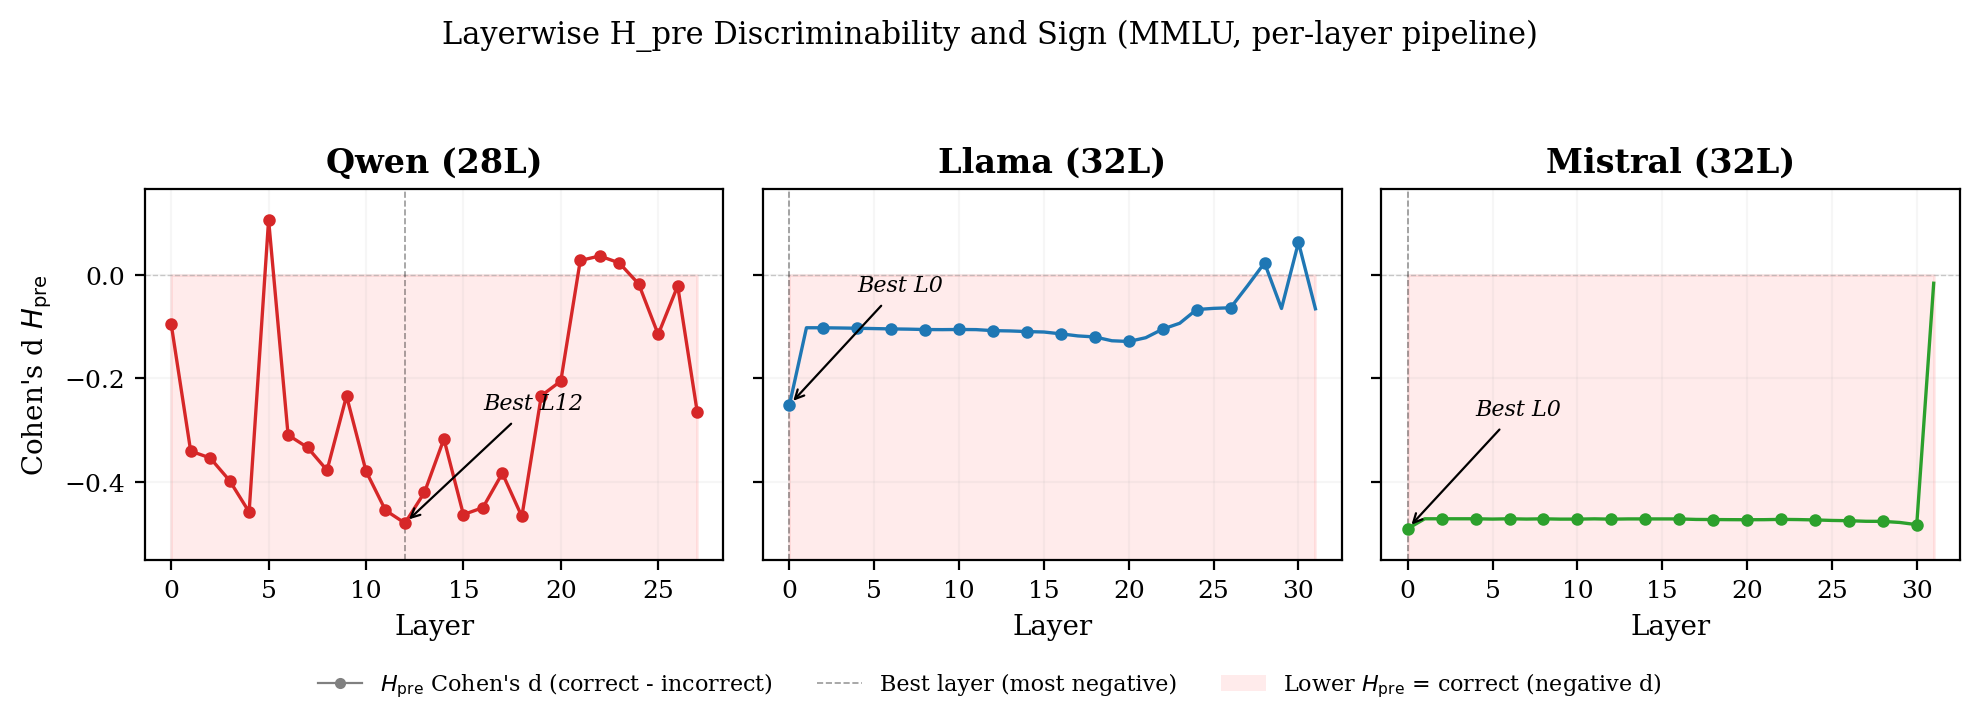
\includegraphics[width=\textwidth]{fig6.png}
\caption{Per-layer $\Hpre$ discrimination (Cohen's $d$; correct $-$ incorrect) across three models on MMLU (full-sample, generation-average). All panels share the same $y$-axis for direct cross-model comparison. No universal $\Hpre$ peak emerges: Qwen shows a wide dynamic range, whereas Llama and Mistral are comparatively flat across most layers. Note: this full-sample Cohen's $d$ visualization uses a different metric and protocol from the held-out AUROC in Table~\ref{tab:baseline}.}
\label{fig:perlayer_d}
\end{figure*}


%===============================================================================
\section{Decoder Faithfulness as a Separate Practical Constraint}
\label{sec:decoder}

\subsection{Raw Logit Lens Poorly Matches the Final-Layer Distribution on Qwen}
\label{sec:faithfulness}

As noted in Section~\ref{sec:definitions}, $\Hpre$ and $\Hpost$ are diagnostic projections that apply the final-layer decoder to intermediate representations. Prior work already observed that raw Logit Lens can be brittle: Tuned Lens achieves uniformly lower bias and perplexity across model families \cite{belrose2023tuned}, and learned linear shortcuts outperform identity projection by 15--40\% in prediction estimation \cite{yomdin2024jump}. We do not present Logit Lens unfaithfulness as our primary contribution. The measurement non-equivalence we identify is a separate concern: for the raw logit lens (linear decoder), the pre-/post-RMSNorm distinction holds exactly; for affine decoders such as Tuned Lens, it holds approximately when decoder-output norms satisfy $\|W_l h\| \gg \|b_l\|$ (see the analysis below). We do not directly benchmark TL-based entropy before versus after RMSNorm in this paper; Section~\ref{sec:tl_control} instead tests whether a more faithful decoder overcomes the scale-ordering pattern observed with the raw logit lens. To assess faithfulness, we train a Tuned Lens (affine translator, 3 epochs on wikitext-2) for each model (see Appendix~\ref{app:tuned} for per-layer KL and top-1 comparisons).

\begin{figure*}[!t]
\centering
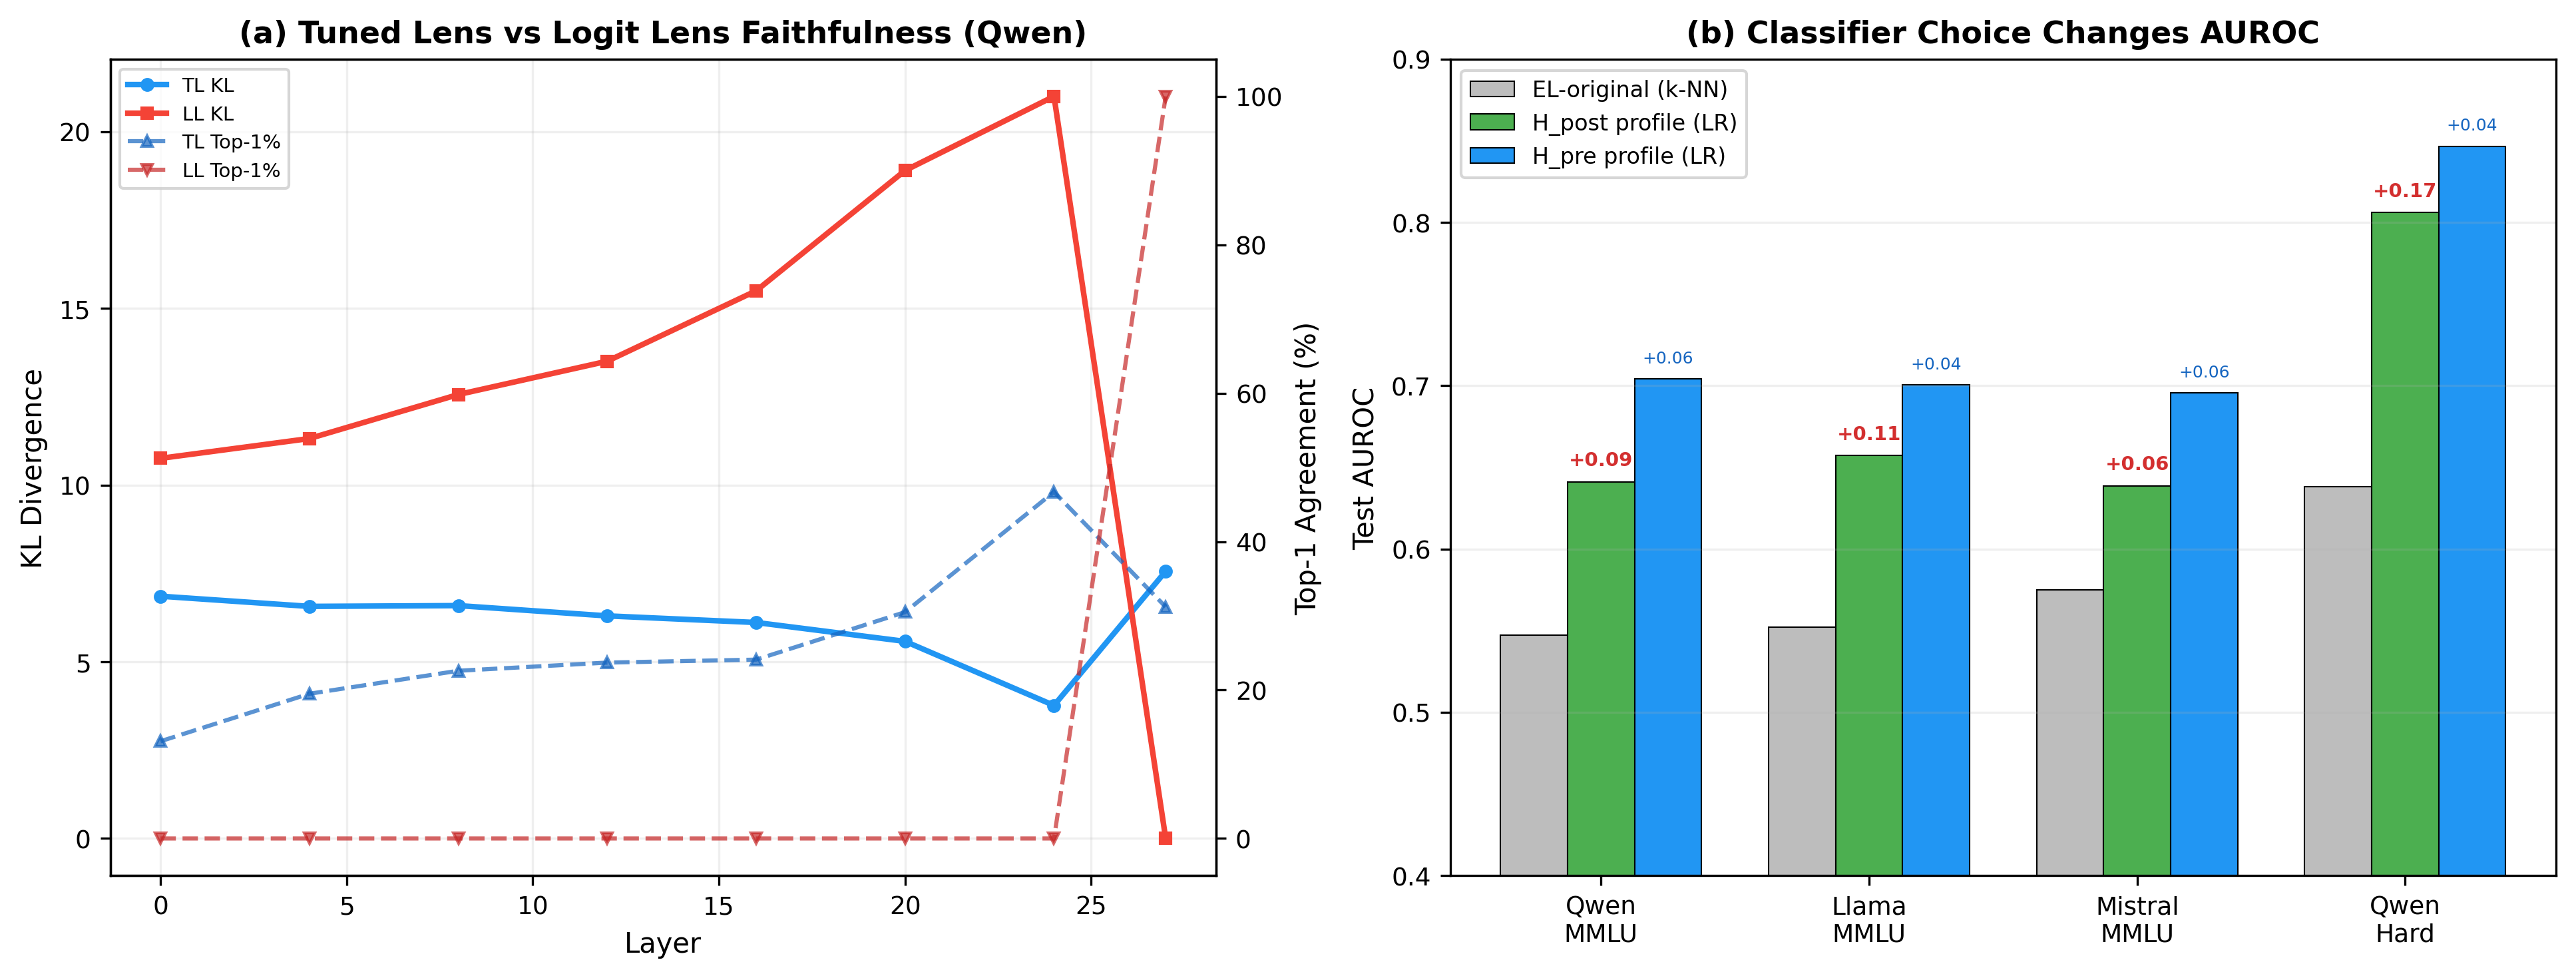
\includegraphics[width=\textwidth]{fig7.png}
\caption{Lens dependence. (a)~Tuned Lens vs.\ Logit Lens faithfulness on Qwen: TL achieves lower Kullback--Leibler (KL) divergence from the final-layer distribution and higher top-1 agreement at all non-final layers, while LL shows 0\% top-1 in middle layers (the final layer, where LL is trivially exact, is excluded from this comparison). (b)~Classifier effect: switching from $k$-NN to LR on identical features increases AUROC by +0.06 to +0.17.}
\label{fig:lens_dependence}
\end{figure*}

On Qwen, Logit Lens achieves 0\% top-1 agreement with the final-layer distribution in middle layers (Fig.~\ref{fig:lens_dependence}a), indicating that $\Hpre$ computed via the raw lm\_head projection is a poor proxy for the final-layer prediction at those layers. Tuned Lens substantially improves faithfulness (KL(TL, final) $<$ KL(LL, final) in 27 of 28 layers; the remaining layer is the final layer, where Logit Lens is trivially exact). The same faithfulness pattern holds across all three model families (Appendix~\ref{app:tuned}). On Qwen MMLU prompt-last (Step~0), Tuned Lens achieves the highest discrimination (AUROC 0.5629 vs.\ Logit Lens 0.5325 vs.\ $\Hpost$ 0.5574), but gains over Logit Lens are modest (+0.030). This does not invalidate $\Hpre$ as a useful correctness discriminator---predictive utility and faithfulness are independent properties. However, it means that $\Hpre$ should not be interpreted as revealing what the model ``believes'' at a given layer. Out-of-sample evaluation on a separate corpus was not performed in this study, so the faithfulness advantage aligns with prior findings but has not been independently validated here. We further test whether TL-based entropy overcomes the scale-redundancy finding in Section~\ref{sec:tl_control}.

The scale-sensitivity distinction between $\Hpre$ and $\Hpost$ holds exactly for any linear decoder (bias = 0), including the raw logit lens. For affine decoders such as the Tuned Lens, which applies $T_l(h) = W_l h + b_l$, the situation is approximate: scaling $h$ by $\alpha$ yields $T_l(\alpha h) = \alpha W_l h + b_l$, which is not a pure temperature rescaling due to the bias term $b_l$. However, when $\|W_l h\| \gg \|b_l\|$ in the logit space (which typically holds in middle and late layers where hidden-state norms are large), the bias becomes negligible and the temperature effect dominates. Applying RMSNorm before $T_l$ would similarly remove radial scale. Thus, the measurement confound identified in this paper is a structural property of RMSNorm that applies to the raw logit lens exactly and to affine decoders approximately in the regime where decoder-output norms are large relative to bias norms.

\subsection{Classifier Choice Changes Discrimination}
\label{sec:classifier}

Reproducing the Entropy-Lens setup ($\Hpost$ profile + $k$-NN, $k$=3) and comparing with the same features under logistic regression reveals a large classifier effect (Fig.~\ref{fig:lens_dependence}b): switching from $k$-NN to LR on the same $\Hpost$ features increases AUROC by +0.06 to +0.17 across conditions (e.g., Qwen Hard: $k$-NN 0.638 $\to$ LR 0.806; Llama MMLU: 0.552 $\to$ 0.657). Under LR, $\Hpre$ profiles further outperform $\Hpost$ profiles in all four conditions (0.70--0.85 vs.\ 0.61--0.81). A natural objection is that this gap might close if $k$-NN hyperparameters were properly tuned. We test this by sweeping $k$ in \{1, 3, 5, 7, 11, 15, 21\} with both euclidean and manhattan distance metrics (5-fold CV, StandardScaler applied). LR still outperforms the best tuned $k$-NN in all 12 profile-model combinations (gap +0.005 to +0.109; full sweep provided in the repository). The classifier effect is therefore not an artifact of using an untuned $k$-NN baseline.

Under a common classifier (LR), $\Hpre$ profile outperforms $\Hpost$ profile in all four sampled-generation conditions (+0.04 to +0.06), reflecting the additional scale information in $\Hpre$.

\subsection{Practical Consequence: Re-evaluating Entropy-Lens Under Normalization Control}
\label{sec:reeval}

The preceding sections establish that $\Hpre$ and $\Hpost$ are non-equivalent measurements with different invariance properties. Does this matter in practice? We test this by revisiting a concrete recent study: Entropy-Lens \cite{ali2025entropylens}, which constructs layerwise entropy profiles and uses them---via $k$-NN classification---to identify ``critical layers'' and classify model ``decision strategies'' (expansion vs.\ pruning). We conduct a systematic re-evaluation using the same MMLU data (Table~\ref{tab:profile_reeval}; 3 models, 1000 samples each, generation-average), comparing $\Hpre$, $\Hpost$, and scale (logit\_std + h\_norm) profiles under both $k$-NN ($k$=3, as in the original) and logistic regression, with 5-fold stratified cross-validation.

\begin{table}[!h]
\centering
\caption{Profile-based correctness AUROC (mean $\pm$ std across folds). All profiles use $L$ features per model (one value per layer) except ``scale'' which uses $2L$ features (logit\_std + h\_norm combined). [Protocol: sampled, gen-avg, 5-fold CV]}
\label{tab:profile_reeval}
\footnotesize
\setlength{\tabcolsep}{1.5pt}
\begin{tabular}{ll ccc}
\toprule
Profile & Clf. & Qwen & Llama & Mistral \\
\midrule
$\Hpre$ & $k$-NN & 0.566$\pm$0.033 & 0.545$\pm$0.062 & 0.567$\pm$0.050 \\
$\Hpre$ & LR & 0.707$\pm$0.038 & 0.683$\pm$0.033 & 0.687$\pm$0.026 \\
$\Hpost$ & $k$-NN & 0.553$\pm$0.050 & 0.559$\pm$0.037 & 0.549$\pm$0.033 \\
$\Hpost$ & LR & 0.698$\pm$0.027 & 0.651$\pm$0.045 & 0.610$\pm$0.045 \\
h\_norm & LR & 0.708$\pm$0.034 & \textbf{0.711$\pm$0.031} & 0.741$\pm$0.028 \\
logit\_std & LR & 0.717$\pm$0.030 & 0.699$\pm$0.026 & 0.744$\pm$0.026 \\
scale & LR & \textbf{0.731$\pm$0.033} & 0.709$\pm$0.026 & \textbf{0.749$\pm$0.027} \\
\bottomrule
\end{tabular}
\end{table}

Even under dimension-matched comparison ($L$ features each), both h\_norm and logit\_std profiles individually outperform $\Hpre$ profiles on all three models (h\_norm: +0.001 to +0.054; logit\_std: +0.010 to +0.058). The combined scale profile (2$L$ features) provides a modest further improvement. The $k$-NN classifier substantially underestimates all profiles (AUROC 0.54--0.57 vs.\ 0.61--0.75 under LR), confirming that classifier choice significantly affects observed discrimination and should be controlled in comparative studies.

\textbf{Scale covariate redundancy.} Adding $\Hpre$ or $\Hpost$ to the combined scale profile yields little incremental utility: deltas range from $-$0.015 to +0.003 across models (Qwen: scale 0.731, +$\Hpre$ $\delta$=$-$0.005; Llama: scale 0.709, +$\Hpre$ $\delta$=$-$0.001; Mistral: scale 0.749, +$\Hpre$ $\delta$=+0.002). This extends the redundancy finding (Table~\ref{tab:incremental}) to full layerwise profiles.

\textbf{Paired fold-wise comparison.} Paired fold-wise differences (scale minus $\Hpre$ AUROC, same 5-fold CV) show that the combined scale profile numerically outperforms $\Hpre$ on all three models under sampled generation: Qwen +0.024 [+0.013, +0.042], Llama +0.025 [+0.009, +0.042], Mistral +0.062 [+0.029, +0.096] (all CIs exclude zero). These intervals are descriptive summaries over $n$=5 non-independent folds and should not be interpreted as formal significance tests. Under greedy decoding, fold-wise support drops from 3/3 to 1/3 models with CIs excluding zero (detailed fold-wise comparisons provided in the repository), indicating that the numerical advantage of scale over entropy weakens under greedy even when profile-level redundancy still holds.

\textbf{Critical layer landscape.} Under the 5-fold CV protocol, the best single-layer for correctness discrimination shifts dramatically between $\Hpre$ and $\Hpost$: Qwen L4$\to$L27 (23 layers), Llama L0$\to$L10 (10 layers), Mistral L0$\to$L24 (24 layers). The argmax shifts are most meaningful on Qwen, where the landscapes are qualitatively different (flat vs.\ peaked); on Llama and Mistral, both are relatively flat, so argmax selections should be interpreted with caution.

However, best-layer argmax comparisons alone overstate the precision of these shifts. Per-layer AUROC analysis with 95\% bootstrap confidence intervals (1000 resamples, full-sample evaluation on MMLU) reveals that $\Hpre$ and $\Hpost$ have qualitatively different per-layer AUROC landscapes (Table~\ref{tab:landscape}):

\begin{table}[!h]
\centering
\caption{Per-layer AUROC landscape and cross-normalization layer penalty (sampled protocol).}
\label{tab:landscape}
\footnotesize
\setlength{\tabcolsep}{3pt}
\begin{tabular}{l cc cc}
\toprule
\multicolumn{5}{l}{\textit{Panel A. Number of layers indistinguishable from best (full-sample bootstrap)}} \\
\midrule
Model & $\Hpre$ indist.\ & $\Hpost$ indist.\ & $\Hpre$ curve & $\Hpost$ curve \\
\midrule
Qwen & 20/28 & 2/28 & Flat plateau & Sharp peak \\
Llama & 29/32 & 24/32 & Nearly flat & Broad \\
Mistral & 31/32 & 29/32 & Nearly flat & Nearly flat \\
\midrule
\multicolumn{5}{l}{\textit{Panel B. AUROC penalty when forced to use the other metric's best layer}} \\
\midrule
Model & $\Hpost$ penalty & 95\% CI & $\Hpre$ penalty & 95\% CI \\
\midrule
Qwen & +0.117 & [{+}.000,{+}.243] & +0.038 & [{-}.059,{+}.143] \\
Llama & +0.040 & [{-}.050,{+}.146] & +0.049 & [{-}.003,{+}.125] \\
Mistral & +0.027 & [{-}.049,{+}.111] & +0.004 & [{-}.004,{+}.012] \\
\bottomrule
\end{tabular}
\end{table}

(``Indistinguishable'' = layer whose 95\% CI upper bound overlaps with the best layer's CI lower bound.)

On Qwen, $\Hpost$ concentrates its discriminative signal in a narrow region (L15--L27), while $\Hpre$ is flat across nearly all layers---the best-layer difference reflects a genuine qualitative distinction in AUROC landscape, not merely argmax instability. On Llama and Mistral, both curves are relatively flat (29/32 and 31/32 layers indistinguishable from best for $\Hpre$, respectively), so the argmax best-layer selections are less statistically meaningful---many layers perform comparably.

\textbf{Sensitivity and stability.} Expansion/pruning strategy labels did not flip between $\Hpre$ and $\Hpost$ in any evaluated sample across all three models (an empirical observation, not a formal invariance guarantee). Three analytical outputs, however, are sensitive to the normalization and classifier choice:

\begin{enumerate}
\item \textbf{The per-layer AUROC landscape differs qualitatively}: $\Hpost$ shows a sharp peak on Qwen (2/28 layers indistinguishable from best) while $\Hpre$ is flat (20/28), leading to substantively different analytical conclusions about which layers carry discriminative information.

\item \textbf{Whether entropy adds information beyond scale changes}: Under the original $k$-NN classifier, $\Hpost$ profiles appear moderately discriminative (AUROC 0.549--0.559). Under LR with scale covariates, entropy profiles provide zero incremental utility (delta $-$0.015 to +0.003), confirmed by the greedy decoding results (delta $-$0.007 to +0.000; Section~\ref{sec:greedy}). Whether entropy is ``informative beyond scale'' depends on whether scale baselines are included.

\item \textbf{Apparent profile AUROC changes with classifier}: Switching from $k$-NN to LR on identical features changes AUROC by +0.06 to +0.17 (Section~\ref{sec:classifier}). The relative ranking of $\Hpre$ vs.\ $\Hpost$ also changes: under $k$-NN, $\Hpost$ slightly outperforms $\Hpre$ on Llama; under LR, $\Hpre$ outperforms $\Hpost$ on all three models.
\end{enumerate}

\textbf{Selective prediction protocol.} For each entropy metric ($\Hpre$ or $\Hpost$), samples are ranked by the generation-average scalar value at the best layer (lower entropy = higher confidence). The top-$c$ fraction is retained (coverage $= c$); selective accuracy is the accuracy on retained samples. At each coverage level, the ``top-ranked model'' is the model with the highest selective accuracy. We sweep $c \in \{0.6, 0.7, 0.8, 0.9\}$, and assess significance via a selection-aware nested bootstrap (2000 iterations; the bootstrap resamples items, re-selects the top-$c$ fraction, and recomputes selective accuracy within each resample).

A fourth sensitive output appears in selective prediction: at fixed 80\% coverage, the top-ranked model label differs between $\Hpre$- and $\Hpost$-based abstention in 20/20 sampled-generation splits and 19/20 greedy splits. However, this ranking instability does not correspond to statistically significant selective-accuracy gains: only 1 of 6 model/protocol cells reached nominal significance under a selection-aware nested bootstrap (Mistral sampled: +3.6~pp, $p = 0.05$, uncorrected). We interpret this as evidence that apparent model ranking can flip on within-noise differences, not that one normalization choice produces meaningfully better selective accuracy. We therefore treat ranking instability, not a universal selective-accuracy gain, as the practical consequence. Full details in Appendix~\ref{app:ranking}.

Normalization and classifier choices alone suffice to change these four analytical outputs on matched data, demonstrating that the analytical framework is sensitive to design choices that were not controlled. The re-evaluation above uses our three primary models under our generation-average protocol; Section~\ref{sec:reproduction} reproduces the analysis on two Entropy-Lens original models under their evaluation protocol.

\FloatBarrier
\subsection{Step 0 Redundancy Confirmation}
\label{sec:step0_redundancy}

To rule out the possibility that $\Hpre$'s scale redundancy is an artifact of generation-length confounding, we replicate the incremental utility test at Step~0 (prompt-last), where no tokens have been generated and length is undefined. On Llama and Mistral, adding $\Hpre$ to scale features yields effectively zero incremental utility at Step~0, matching the generation-average results. On Qwen, the delta is positive but comparable in magnitude to the AUROC standard deviation across 20 repeated splits (0.022--0.031; Appendix~\ref{app:repeated}). The key finding is that scale redundancy also appears at Step~0 in two of the three models, which reduces the likelihood that the main result is driven only by generation length. Full Step~0 results are in Appendix~\ref{app:token}.

\subsection{Tuned Lens Control: Scale Ordering Under a More Faithful Decoder}
\label{sec:tl_control}

As a robustness control, we test whether a more faithful decoder changes the observed scale-entropy ordering. Sections~\ref{sec:predictive} established that scale proxies match or outperform $\Hpre$ under the raw logit lens. A natural objection is that this might be an artifact of logit-lens unfaithfulness: if the raw decoder fails to capture meaningful distributional content, perhaps a more faithful decoder would yield entropy that outperforms scale. We test this directly by computing Tuned Lens entropy ($\Htl$) for each layer and evaluating its correctness discrimination under the same held-out protocol, across all three model families.

For each model, Tuned Lens affine translators were trained on wikitext-2 (Section~\ref{sec:faithfulness}, Appendix~\ref{app:tuned}). We then compute $\Htl$ at every layer for each MMLU sample (1000 per model, same items as the baseline evaluation), select the best layer and sign on the calibration set, and evaluate on the held-out test set.

Under this setup (independent generation run, not directly comparable to Table~\ref{tab:baseline}; full results provided in the repository), all metrics---including $\Htl$, $\Hpre$, and scale baselines---cluster near chance level (AUROC 0.45--0.52), so $\Htl$ does not outperform the best scale proxy in any of the three models. Adding $\Htl$ to logit\_std yields negligible or negative incremental utility across all three models---on Llama and Mistral, $\Htl$ \textit{decreases} discrimination, indicating that Tuned Lens entropy does not provide complementary information beyond scale.

\textbf{Step 0 (prompt-last) results.} The same pattern holds at Step~0: $\Htl$ is outperformed by at least one scale proxy (h\_norm or logit\_std) in all three models.

\textbf{Interpretation.} This result is inconclusive rather than negative: all metrics cluster within AUROC 0.45--0.52 on this independent run, so the experiment lacks power to adjudicate the scale-entropy ordering. The TL control shows only that scale-correlated redundancy was not broken by this particular decoder in this setup; stronger decoders---longer training, task-matched data, or methods such as SimLens \cite{ma2025simlens}---remain untested (Section~\ref{sec:future}).

\subsection{Protocol-Matched Reproduction on Entropy-Lens Original Models}
\label{sec:reproduction}

As targeted corroboration, we reproduce the analysis on two Entropy-Lens original models (Llama-3-8B-Instruct and Llama-3.2-3B-Instruct) under a protocol matching five key design choices from Ali et al.\ \cite{ali2025entropylens}: 1-shot MMLU, 32-token entropy averaging, $k$-NN ($k$=3), 10-fold CV, and logit-based answer extraction (full details in Appendix~\ref{app:reproduction}). The main findings replicate: scale profiles outperform entropy profiles under LR on Llama-3-8B (0.668 vs.\ 0.617/0.620), classifier switching from $k$-NN to LR increases AUROC by +0.04 to +0.09, and the best discriminative layer shifts by 17--19 layers between $\Hpre$ and $\Hpost$. The one partial exception is Llama-3.2-3B, where $\Hpre$ LR (0.606) exceeds scale LR (0.576) by +0.030---the only model where entropy outperforms scale, occurring in a low-discrimination regime (all AUROCs 0.50--0.61). Including these results, the main findings generalize across four models spanning three families under two independent protocols.


%===============================================================================
\FloatBarrier
\section{Discussion, Limitations, and Reporting Recommendations}
\label{sec:discussion}

\subsection{Implications for Prior Work}
\label{sec:implications}

Our findings have implications for studies that compute entropy from logit-lens projections. The measurement non-equivalence documented in this paper (Sections~\ref{sec:what}, \ref{sec:reeval}) means that studies reporting ``layerwise entropy'' without specifying $\Hpre$ vs.\ $\Hpost$ may be measuring hidden-state scale, directional content, or some mixture of both. As illustrative context for nearby reporting practices (not a systematic review or a basis for invalidating specific prior results), Table~\ref{tab:litaudit} surveys how representative prior work handles this specification.

\FloatBarrier
\begin{table*}[!t]
\centering
\caption{Representative literature audit (illustrative, not systematic): normalization specification in prior work on layerwise entropy / internal uncertainty. Panel~A: Intermediate vocabulary projection (logit-lens family). Panel~B: Probe-based, output-level, or other internal methods.}
\label{tab:litaudit}
\begin{tabular}{l l c c c}
\toprule
Reference & Lens / method & Norm.\ specified? & Scale baseline? & Evidence \\
\midrule
\multicolumn{5}{l}{\textit{Panel A. Intermediate vocabulary projection (logit-lens family)}} \\
\midrule
nostalgebraist \cite{nostalgebraist2020logitlens} & Logit Lens & Unspecified & No & Text \\
Belrose et al.\ \cite{belrose2023tuned} & Tuned Lens & Yes (explicit) & No & Text + formula \\
Ali et al.\ \cite{ali2025entropylens} & Entropy-Lens & Text unspec.; code applies LN & No & Text + code \\
Geva et al.\ \cite{geva2022transformer} & FF vocab proj. & Explicitly omitted & No & Text + appendix \\
Chuang et al.\ \cite{chuang2024dola} & DoLa & Not specified & No & Text \\
Ma et al.\ \cite{ma2025simlens} & SimLens & Not specified & No & Text \\
Lad et al.\ \cite{lad2024robustness} & Logit-lens entropy & Not specified & No & Text \\
Qiu et al.\ \cite{qiu2025entropy} & Entropy layer contrast & Not specified & No & Text + formula \\
Das et al.\ \cite{das2025entropy} & Entropy-guided selection & Not specified & No & Text + formula \\
\midrule
\multicolumn{5}{l}{\textit{Panel B. Probe-based, output-level, or other internal methods}} \\
\midrule
Kossen et al.\ \cite{kossen2024seps} & SEPs (probe) & N/A & No & Text \\
Bhatnagar et al.\ \cite{bhatnagar2026drift} & DRIFT (probe) & N/A & No & Text \\
Gao et al.\ \cite{gao2025flue} & FLUE (hidden-state H) & N/A & N/A & Text \\
Chen et al.\ \cite{chen2025querylevel} & Internal Conf.\ (pre-gen.) & N/A & No & Text \\
Stolfo et al.\ \cite{stolfo2024confidence} & Conf.\ Reg.\ Neurons & Partial (norm-based) & Partial & Text \\
\bottomrule
\end{tabular}
\end{table*}

Among the nine Panel~A works, normalization handling is inconsistent: two explicitly specify their choice (Belrose et al.\ include LayerNorm; Geva et al.\ omit it and verify in an appendix), one applies LayerNorm in code but not in the main text \cite{ali2025entropylens}, and the remaining six do not specify the normalization point. None report direct scale baselines alongside entropy. Panel~B uses probe-based or output-level methods where the normalization point is less directly relevant.

This cross-paper variation does not imply that any individual finding is invalid, but it does mean that the normalization-dependent measurement choice has not been consistently specified or controlled for. We discuss three categories of research for which the normalization point is a relevant diagnostic variable below; without matched re-evaluation under both $\Hpre$ and $\Hpost$, we do not claim that any specific prior conclusion is incorrect.

\textbf{Logit-lens entropy without normalization specification.} The logit lens \cite{nostalgebraist2020logitlens} projects intermediate hidden states to vocabulary space via the language model head. When researchers compute entropy from these projections without specifying whether the hidden state is first normalized, our results indicate that pre-normalization decoded entropy responds to hidden-state magnitude and can be strongly influenced by scale (Section~\ref{sec:what}). The degree of cross-sample norm dominance is model-dependent: Llama and Mistral show strong radial coupling ($R^2 > 0.82$), whereas Qwen retains substantial directional variation ($R^2 \approx 0.15$) despite remaining functionally scale-sensitive under intervention (Section~\ref{sec:radial_angular}). Specifically, in RMSNorm-based models, pre-normalization logit-lens entropy acts as an implicit temperature-scaled measure: for fixed direction, layers with large hidden-state norms produce concentrated distributions (low entropy), while layers with small norms produce near-uniform distributions (high entropy). Any ``critical layer'' identified by such entropy may reflect a norm magnitude transition rather than a distributional uncertainty shift. We suggest that future work reporting layerwise entropy patterns from logit-lens projections specify whether normalization was applied before the projection.

\textbf{Entropy-Lens and related profiling methods.} Entropy-Lens \cite{ali2025entropylens} constructs entropy profiles across layers and uses them for decision-strategy classification. Our results show that the discriminative content of such profiles depends on the classifier (Section~\ref{sec:classifier}): switching from $k$-NN to logistic regression on the same $\Hpost$ features changes AUROC by up to +0.17. Furthermore, under a common classifier (LR), $\Hpre$ profiles outperform $\Hpost$ profiles in all four conditions (+0.04 to +0.06), reflecting the additional scale information in $\Hpre$. This means that prior comparisons of entropy profiles that do not control for classifier choice may conflate feature quality with classifier suitability---and profiles that appear effective may be leveraging scale information rather than directional uncertainty.

\textbf{Internal uncertainty estimation more broadly.} Methods that extract uncertainty signals from intermediate hidden states---including probing-based approaches \cite{kossen2024seps, bhatnagar2026drift}---may wish to check whether their signals are partially confounded with hidden-state scale, though the relevance depends on whether and how intermediate representations are decoded to vocabulary space. Our norm-binned control analysis (Appendix~\ref{app:normbinned}) provides a diagnostic heuristic: if a signal's AUROC drops substantially after binning by h\_norm or logit\_std, scale dependence is indicated, though binning on a correlated control is indicative rather than definitive. We recommend that future internal-uncertainty work report such controlled baselines alongside raw performance.

\textbf{Decoder design and normalization choice as separate axes.} Post-Logit-Lens methods improve decoded representations along non-equivalent axes: learned translators improve faithfulness \cite{belrose2023tuned, yomdin2024jump}, prompt-mediated frameworks broaden extraction \cite{ghandeharioun2024patchscopes, pal2023futurelens}, and task-specific decoders improve factuality or early-exit utility \cite{chuang2024dola, ma2025simlens}. However, none of these methods explicitly compares pre- and post-RMSNorm projection loci as a measurement variable. Our Tuned Lens control (Section~\ref{sec:tl_control}) provides preliminary evidence in this direction: under our TL setup, scale-correlated redundancy persisted across all three model families. Hernandez et al. \cite{hernandez2024linearity} independently observe that layer normalization causes their linear relational embedding weights to underestimate magnitude changes, introducing a scalar correction $\beta$ to compensate---further evidence that normalization-induced scale effects are a separate concern from decoder fidelity. We therefore suggest that decoder design and normalization choice be treated as separate methodological axes.

\textbf{Known exceptions to scale redundancy.} While scale redundancy holds across the primary 3-model MMLU settings under sampled generation, four exceptions are noted: (i)~Mistral full-feature set yields a nominal-level $\Hpre$ delta of +0.016 (CI [+0.005, +0.029]) that does not survive Bonferroni correction across the eight primary tests; (ii)~Llama-3.2-3B shows $\Hpre$ incremental delta of +0.024 in a low-discrimination regime; (iii)~Qwen Step~0 full-feature set shows +0.047, comparable to partition variance; (iv)~TruthfulQA mc1 shows +0.016 on a single model. Under greedy decoding, profile-level redundancy holds numerically (deltas $-$0.007 to +0.000) but statistical support drops from 3/3 to 1/3 models with CIs excluding zero. These exceptions indicate that scale redundancy is a predominant pattern in the tested settings rather than a universal law.

These implications are bounded by our experimental scope: three 7--8B RMSNorm-based models on mathematical reasoning and MMLU. Whether analogous confounds arise in LayerNorm-based architectures, larger models, or open-ended generation tasks remains an open empirical question. Concurrent work by Mar\'in \cite{marin2026rotational} independently distinguishes normalized from raw logit-lens projections and reports that applying final normalization stabilizes early-layer decoding; our work complements this by systematically characterizing how this choice changes what decoded entropy measures across three model families. We frame these as diagnostic considerations rather than definitive invalidations of prior findings.

\subsection{Scope and Boundaries}

\begin{enumerate}
\item Normalization qualitatively changes what decoded entropy emphasizes under the chosen projection.
\item $\Hpre$ is scale-sensitive by construction; $\Hpost$ is largely scale-invariant outside low-norm early layers.
\item Scale baselines match or exceed single-layer entropy for correctness discrimination under both sampled and greedy protocols; repeated-split stability degrades under greedy (Appendix~\ref{app:greedy}).
\item Internal-layer signals match or exceed final-output entropy; margins range from +0.001 (Qwen greedy) to +0.255 (Mistral greedy).
\item Analytical conclusions depend on layer, token position, model family, and decoding lens.
\item Cross-study comparability requires normalization specification.
\end{enumerate}

\noindent This paper does not identify reasoning layers, claim causal mediation, or propose $\Hpre$ as a universal uncertainty estimator. Scale redundancy is demonstrated under the protocols studied here, not for every downstream use of decoded entropy.

\subsection{Limitations}

\begin{itemize}
\item \textbf{Model coverage and task scope}: Deep analysis (scale interventions, token positions, multi-seed check) is primarily on Qwen2.5-7B; Llama and Mistral serve as cross-family confirmation on MMLU, not full replications. A preliminary TruthfulQA extension (Appendix~\ref{app:truthfulqa}) suggests slightly weaker scale redundancy on factual-knowledge tasks. Whether findings extend to open-ended generation, larger models, or LayerNorm-based architectures remains open.

\item \textbf{Robustness and protocol sensitivity}: Main results use a single 70/30 split (seed~=~42). Repeated-split analysis (20 splits; Appendix~\ref{app:repeated}) confirms $\Hpre$ sign stability under sampled generation (20/20) but shows layer variability. Under greedy decoding, single-layer sign stability degrades (10--13/20; Appendix~\ref{app:greedy}); profile-level results should be preferred. Multi-seed checks preserve profile-level ordering but show run-to-run AUROC variation.

\item \textbf{Decoder faithfulness}: Both $\Hpre$ and $\Hpost$ apply the final-layer decoder to intermediate representations unfaithfully in middle layers (Section~\ref{sec:faithfulness}). Entropy values should not be interpreted as reflecting the model's latent prediction. The $\Hpost$ alpha-variation in low-norm early layers has not been fully disentangled from finite-precision effects.

\item \textbf{Statistical power}: Coverage comparison $p$-values should be treated as indicative. The Entropy-Lens reproduction (Section~\ref{sec:reproduction}) differs in sample selection and temperature; on Llama-3.2-3B, a modest exception (+0.024) is observed in a low-discrimination regime. On Llama and Mistral, $\Hpre$ ceiling effects limit observable dynamic range.

\item \textbf{Multiple-comparison burden}: This manuscript reports numerous robustness analyses; some findings should be interpreted with multiple-comparison caution, as family-wise correction has not been applied across all tests.

\item \textbf{Literature audit methodology}: Table~\ref{tab:litaudit} is a representative audit of normalization specification practices, not a systematic review; selection and coding judgments are involved, and the sample is not exhaustive.

\item \textbf{Evaluation label noise}: Answer extraction and correctness labeling from model outputs could affect AUROC estimates, particularly in low-accuracy regimes.
\end{itemize}

\FloatBarrier
\subsection{Reporting Recommendations}
\label{sec:recommendations}

Based on our findings, we recommend that future work on layerwise entropy adopt the practices condensed in Table~\ref{tab:checklist}. Items 1--3 address the measurement confound: (1)~specify whether entropy is pre- or post-normalization, since the two measure qualitatively different quantities; (2)~include scale baselines (logit\_std, h\_norm) to test whether entropy is scale-dominated---the norm-binned diagnostic (Appendix~\ref{app:normbinned}) provides a concrete test; (3)~calibrate sign and best layer on a held-out set, since the entropy-correctness sign can reverse across families (Section~\ref{sec:sign_reversal}) and the best layer is condition-dependent. Items 4--6 address methodological pitfalls: (4)~specify token position, as different metrics favor different positions (Section~\ref{sec:token_position}); (5)~control both decoder and classifier, since classifier choice alone shifts AUROC by up to +0.17 (Section~\ref{sec:classifier}); (6)~report $\epsilon$ and gain parameters, as these affect early-layer behavior (Section~\ref{sec:epsilon}).

\begin{table}[!h]
\centering
\caption{Diagnostic reporting checklist.}
\label{tab:checklist}
\begin{tabular}{c l}
\toprule
\# & Item \\
\midrule
1 & Normalization point (pre- or post-) specified \\
2 & Scale baselines (logit\_std, h\_norm) reported alongside entropy \\
3 & Sign direction and best layer calibrated on held-out set \\
4 & Token position specified \\
5 & Decoder lens and classifier controlled \\
6 & Normalization details ($\epsilon$, gain) noted \\
\bottomrule
\end{tabular}
\end{table}

This checklist is a practical aid for cross-study comparability, not a mandatory standard.

\FloatBarrier
\subsection{Future Work}
\label{sec:future}

\begin{itemize}
\item Extending to LayerNorm-based architectures, larger models, and multi-seed robustness on Llama and Mistral to strengthen cross-family evidence.
\item Evaluation on open-ended generation, code generation, and long-form QA. $\Hpost$ may prove more informative where scale carries less task-relevant information, such as out-of-distribution or hallucination detection.
\item Investigation of more faithful decoders (e.g., SimLens \cite{ma2025simlens}, non-linear or task-specific decoders) under matched classifiers. Our TL control did not break scale-correlated redundancy, but alternative decoders remain untested.
\end{itemize}


%===============================================================================
\section{Conclusion}
\label{sec:conclusion}

In the three 7--8B RMSNorm-based decoder LMs studied here, measuring entropy before versus after the final RMSNorm yields non-equivalent diagnostic signals. $\Hpre$ is mathematically scale-sensitive by construction, and our interventions confirm that this sensitivity is empirically large; $\Hpost$ is largely scale-invariant in middle and late layers. Scale proxies match or exceed single-layer entropy for correctness discrimination in the tested conditions, per-layer AUROC landscapes differ qualitatively between $\Hpre$ and $\Hpost$, and classifier choice alone shifts apparent AUROC by up to +0.17. These findings hold under both sampled and greedy protocols, though statistical support weakens under greedy decoding. The correlational composition of $\Hpre$ is itself model-dependent ($R^2 \approx 0.15$ in Qwen vs.\ $R^2 > 0.82$ in Llama and Mistral), indicating that scale redundancy and scale sensitivity operate through partially independent mechanisms.

We offer a six-item reporting checklist (Table~\ref{tab:checklist}): specify the normalization point, report direct scale baselines, calibrate sign and layer on held-out data, specify token position, control decoder and classifier choice, and report normalization implementation details. Our claims concern decoder-dependent post-generation diagnostics under the raw logit lens in the tested settings, and should not be generalized beyond these models, tasks, or protocols without further evidence. The present work is a methodological contribution: it informs how researchers should measure and report layerwise entropy rather than proposing a deployable uncertainty estimator.

\section*{Code and Data Availability}

All code, Tuned Lens parameters, result files, manifests, and reproduction scripts are available at \url{https://github.com/sungmoon2/Normalization-Changes-LLM-Entropy} (commit: \texttt{4468610}). Datasets (MMLU, competition\_math, TruthfulQA) and model weights (Qwen2.5-7B-Instruct, Llama-3-8B-Instruct, Mistral-7B-Instruct-v0.3) are publicly available through HuggingFace under their respective licenses.

%===============================================================================
\FloatBarrier
\appendices

\section{Additional Evaluation Conditions}
\label{app:additional}

Three supplementary conditions were evaluated under separate experimental pipelines and are \textbf{not directly comparable} to the main held-out results in Tables~\ref{tab:baseline}--\ref{tab:incremental}. We report available metrics below for reference.

\textbf{Qwen Easy (competition\_math Level 1--2, 500 samples drawn, 400 valid after NaN filtering, accuracy 85.25\% = 341/400).} Evaluated under an earlier, non-main pipeline. Available AUROC values (e.g., $\Hpre$ = 0.7295, $\Hpost$ = 0.5757) are provided in the repository.

\textbf{Qwen ARC (ARC-Challenge, 1,119 samples, accuracy 89.3\% = 999/1,119).} Evaluated in separate entropy experiments using full-sample Cohen's $d$ (unnormalized optimal layer L27, $d$ = 0.41) but was not included in the held-out baseline protocol. The high accuracy (89.3\%) limits discriminative dynamic range.

\textbf{Llama Hard (competition\_math Level 4--5, 500 samples, accuracy 9.8\%).} Evaluated with full-sample Cohen's $d$ (normed optimal L9, $d$ = $-$0.42; unnormed optimal L1, $d$ = +0.86). The extreme class imbalance (9.8\% correct) makes held-out AUROC unreliable and was therefore not computed under the main protocol.

\FloatBarrier
\section{Decoder Controls and Scale Intervention Details}
\label{app:tuned}
\label{app:decoder_controls}

\subsection{Tuned Lens Training}

Table~\ref{tab:faithfulness_cross} summarizes cross-model faithfulness. Per-layer affine translators ($W_l$, $b_l$) were trained on wikitext-2 validation set for 3 epochs using Adam (lr=$10^{-3}$) with KL divergence loss. Training results: Qwen 27 layers, loss 7009$\to$2459, TL$>$LL in 27/28; Llama 31 layers, loss 7638$\to$1480, TL$>$LL in 31/32; Mistral 31 layers, loss 3046$\to$843, TL$>$LL in 31/32. TL-based correctness discrimination was evaluated under both Step~0 and generation-average protocols (Section~\ref{sec:tl_control}).

\begin{table}[!h]
\centering
\caption{Cross-model Tuned Lens faithfulness (in-sample, WikiText-2 \cite{merity2016wikitext} validation). TL $>$ LL counts include the final layer (where LL is trivially exact); KL and Top-1 ranges exclude the final layer. TL is trained on layers 0 through $L$--2 only.}
\label{tab:faithfulness_cross}
\footnotesize
\setlength{\tabcolsep}{1.5pt}
\begin{tabular}{l c c cc cc}
\toprule
Model & TL$>$LL & Loss (sum KL) & KL(TL) & KL(LL) & Top-1(TL) & Top-1(LL) \\
\midrule
Qwen & 27/28 & 7009$\to$2459 & 3.8--6.9 & 10.8--21.0 & 13--47\% & 0--0\% \\
Llama & 31/32 & 7638$\to$1480 & 2.8--6.7 & 5.8--10.5 & 18--51\% & 0--67\% \\
Mistral & 31/32 & 3046$\to$843 & 1.8--5.1 & 7.5--8.9 & 15--58\% & 0--77\% \\
\bottomrule
\end{tabular}
\end{table}

On Qwen, Logit Lens achieves 0\% top-1 agreement with the final-layer distribution in middle layers (L4--L24), while Tuned Lens achieves 19--47\%. KL divergence: TL range 3.8--6.9 vs.\ LL range 10.8--21.0 across layers. Llama and Mistral show gradual LL improvement in late layers (up to 67\% and 77\% top-1), while TL reaches 51\% and 58\%.

\subsection{Qwen Scale Intervention Details}

Table~\ref{tab:unitnorm_qwen} provides per-layer intervention values.

\begin{table}[!h]
\centering
\caption{Qwen scale intervention details (competition\_math Hard, 500 samples, Step~0).}
\label{tab:unitnorm_qwen}
\footnotesize
\setlength{\tabcolsep}{2.5pt}
\begin{tabular}{c cc c cc c}
\toprule
\multicolumn{7}{l}{\textit{Panel A. Unit-norm removal}} \\
\midrule
Layer & $\Hpre$ orig & $\Hpre$ unit & $\Delta$ & $\Hpost$ orig & $\Hpost$ unit & $\Delta$ \\
\midrule
0 & 0.9963 & 1.0000 & +0.004 & 0.4788 & 0.4812 & +0.002 \\
4 & 0.9705 & 1.0000 & +0.030 & 0.0780 & 0.0786 & +0.001 \\
12 & 0.8577 & 1.0000 & +0.142 & 0.0484 & 0.0491 & +0.001 \\
16 & 0.6637 & 0.9999 & +0.336 & 0.1822 & 0.1843 & +0.002 \\
24 & 0.0444 & 0.9999 & +0.955 & 0.0861 & 0.0864 & +0.000 \\
27 & 0.0166 & 1.0000 & +0.983 & 0.0307 & 0.0308 & +0.000 \\
\midrule
\multicolumn{7}{l}{\textit{Panel B. Alpha-sweep at representative layers}} \\
\midrule
$\alpha$ & L4 $\Hpre$ & L4 $\Hpost$ & L16 $\Hpre$ & L16 $\Hpost$ & & \\
\midrule
0.25 & 0.9985 & 0.0780 & 0.9817 & 0.1822 & & \\
1.00 & 0.9705 & 0.0780 & 0.6637 & 0.1822 & & \\
4.00 & 0.5169 & 0.0780 & 0.0990 & 0.1822 & & \\
\bottomrule
\end{tabular}
\end{table}

Under alpha-sweep ($\alpha$ 0.25--4.0), mid-layer $\Hpre$ dynamic range is wide for Qwen (L14: 0.058--0.982, range 0.924) but at ceiling for Llama (L16: 0.992--1.000, range 0.008) and Mistral (L16: 0.9995--1.0000, range 0.0005). Full per-layer alpha-sweep tables for Llama and Mistral are provided in the repository; the paper reports only the summarized cross-model pattern (Table~\ref{tab:crossmodel}). The independent-run Tuned Lens control (near-chance AUROCs for all metrics) is also provided in the repository for transparency.


\section{Norm-Binned Controls}
\label{app:normbinned}

Table~\ref{tab:normbinned_hnorm} reports norm-binned retention results. To test whether $\Hpre$'s discrimination is merely a proxy for hidden-state norm or logit variability, we bin samples into 5 equal-frequency groups by the control variable, compute $\Hpre$ AUROC within each bin, and measure weighted retention relative to the original (unbinned) $\Hpre$ AUROC. Retention is defined as $(\text{AUROC}_{\text{binned}} - 0.5) / (\text{AUROC}_{\text{original}} - 0.5) \times 100\%$, where 0.5 represents chance-level AUROC.

\begin{table}[!h]
\centering
\caption{Scale-binned AUROC retention: $\Hpre$ AUROC within 5 equal-frequency bins of the control variable, relative to the unbinned original. This is a diagnostic heuristic, not a formal independence test. [Protocol: sampled, gen-avg]}
\label{tab:normbinned_hnorm}
\footnotesize
\setlength{\tabcolsep}{3pt}
\begin{tabular}{l l ccc}
\toprule
Condition & Control & Orig. & Binned & Ret. \\
\midrule
Qwen Hard & h\_norm & 0.7672 & 0.6121 & 42.0\% \\
Qwen MMLU & h\_norm & 0.6367 & 0.5888 & 65.0\% \\
Llama MMLU & h\_norm & 0.6021 & 0.4564 & $-$42.7\% \\
Mistral MMLU & h\_norm & 0.6737 & 0.6480 & 85.2\% \\
\midrule
Qwen Hard & logit\_std & 0.7672 & 0.4617 & $-$14.3\% \\
Qwen MMLU & logit\_std & 0.6367 & 0.5576 & 42.1\% \\
Llama MMLU & logit\_std & 0.6021 & 0.5347 & 34.0\% \\
Mistral MMLU & logit\_std & 0.6737 & 0.6739 & 100.1\% \\
\bottomrule
\end{tabular}
\end{table}

Mistral $\Hpre$ retains 100.1\% of its AUROC after controlling for logit\_std, consistent with $\Hpre$ being at ceiling (Section~\ref{sec:saturation}): when $\Hpre$ is already saturated, controlling for logit\_std does not reduce $\Hpre$'s signal because both carry the same (minimal) information. Negative retention (Llama $\Hpre$ controlled by h\_norm, Qwen Hard $\Hpre$ controlled by logit\_std) indicates that within-bin $\Hpre$ performance falls below chance, suggesting strong collinearity between the control variable and $\Hpre$ in those conditions.


\FloatBarrier
\section{Token Position Ablations}
\label{app:token}

Table~\ref{tab:token_full} and Fig.~\ref{fig:token_position} report the token-position ablation results. The ablation uses the same 1000 MMLU items as the baseline evaluation (Section~\ref{sec:predictive}), selected via identical \texttt{np.random.choice} sampling (seed~=~42). Item ordering was verified to match exactly across all three models (0/57 MMLU subject-category distribution mismatches per model). Because generation is stochastic (temperature~=~0.3), model responses differ across runs; Qwen achieved the same accuracy (74.9\%), while Llama achieved 65.5\% (vs.\ 63.8\% in the baseline) and Mistral 62.7\% (matching the baseline). The 70/30 calibration/test split uses \texttt{np.random.permutation} (seed~=~42), which differs from the \texttt{StratifiedShuffleSplit} used in the main baseline protocol. Because all comparisons within each token-position condition use the same split, relative metric comparisons remain valid.

\begin{table}[!h]
\centering
\caption{Held-out test AUROC by token position (3 models, MMLU 1000, 70/30 split, same samples as baseline). [Protocol: sampled, 70/30 split]}
\label{tab:token_full}
\footnotesize
\setlength{\tabcolsep}{3pt}
\begin{tabular}{l cccc}
\toprule
\multicolumn{5}{c}{\textbf{Qwen} (n=1000, acc=74.9\%)} \\
\midrule
Metric & Step 0 & Step 1 & Full Avg & Best \\
\midrule
$\Hpre$ & 0.6750 & 0.6036 & \textbf{0.6790} & Full Avg \\
$\Hpost$ & 0.6035 & 0.6509 & \textbf{0.6999} & Full Avg \\
logit\_std & 0.6245 & 0.5938 & \textbf{0.6553} & Full Avg \\
h\_norm & 0.5837 & 0.5291 & \textbf{0.7001} & Full Avg \\
\midrule
\multicolumn{5}{c}{\textbf{Llama} (n=1000, acc=65.5\%)} \\
\midrule
$\Hpre$ & 0.5571 & 0.6628 & \textbf{0.6836} & Full Avg \\
$\Hpost$ & 0.5964 & \textbf{0.6354} & 0.5851 & Step 1 \\
logit\_std & 0.5427 & 0.6623 & \textbf{0.6869} & Full Avg \\
h\_norm & 0.6504 & 0.6554 & \textbf{0.7288} & Full Avg \\
\midrule
\multicolumn{5}{c}{\textbf{Mistral} (n=1000, acc=62.7\%)} \\
\midrule
$\Hpre$ & 0.5517 & 0.6204 & \textbf{0.6757} & Full Avg \\
$\Hpost$ & 0.5874 & \textbf{0.6514} & 0.5723 & Step 1 \\
logit\_std & 0.6321 & 0.5645 & \textbf{0.6734} & Full Avg \\
h\_norm & 0.5582 & 0.6127 & \textbf{0.6643} & Full Avg \\
\bottomrule
\end{tabular}
\end{table}

Full-generation average yields the highest AUROC in 10 of 12 model-metric combinations. $\Hpost$ is the exception on Llama and Mistral, where Step~1 is optimal. Step~0 (pre-generation) carries above-chance signal in all 12 conditions (AUROC 0.54--0.68).

Exact best-layer and sign selections for all conditions are provided in the repository. The repeated-split analysis (Appendix~\ref{app:repeated}) reports modal layer selections across 20 splits.

\begin{figure*}[!t]
\centering
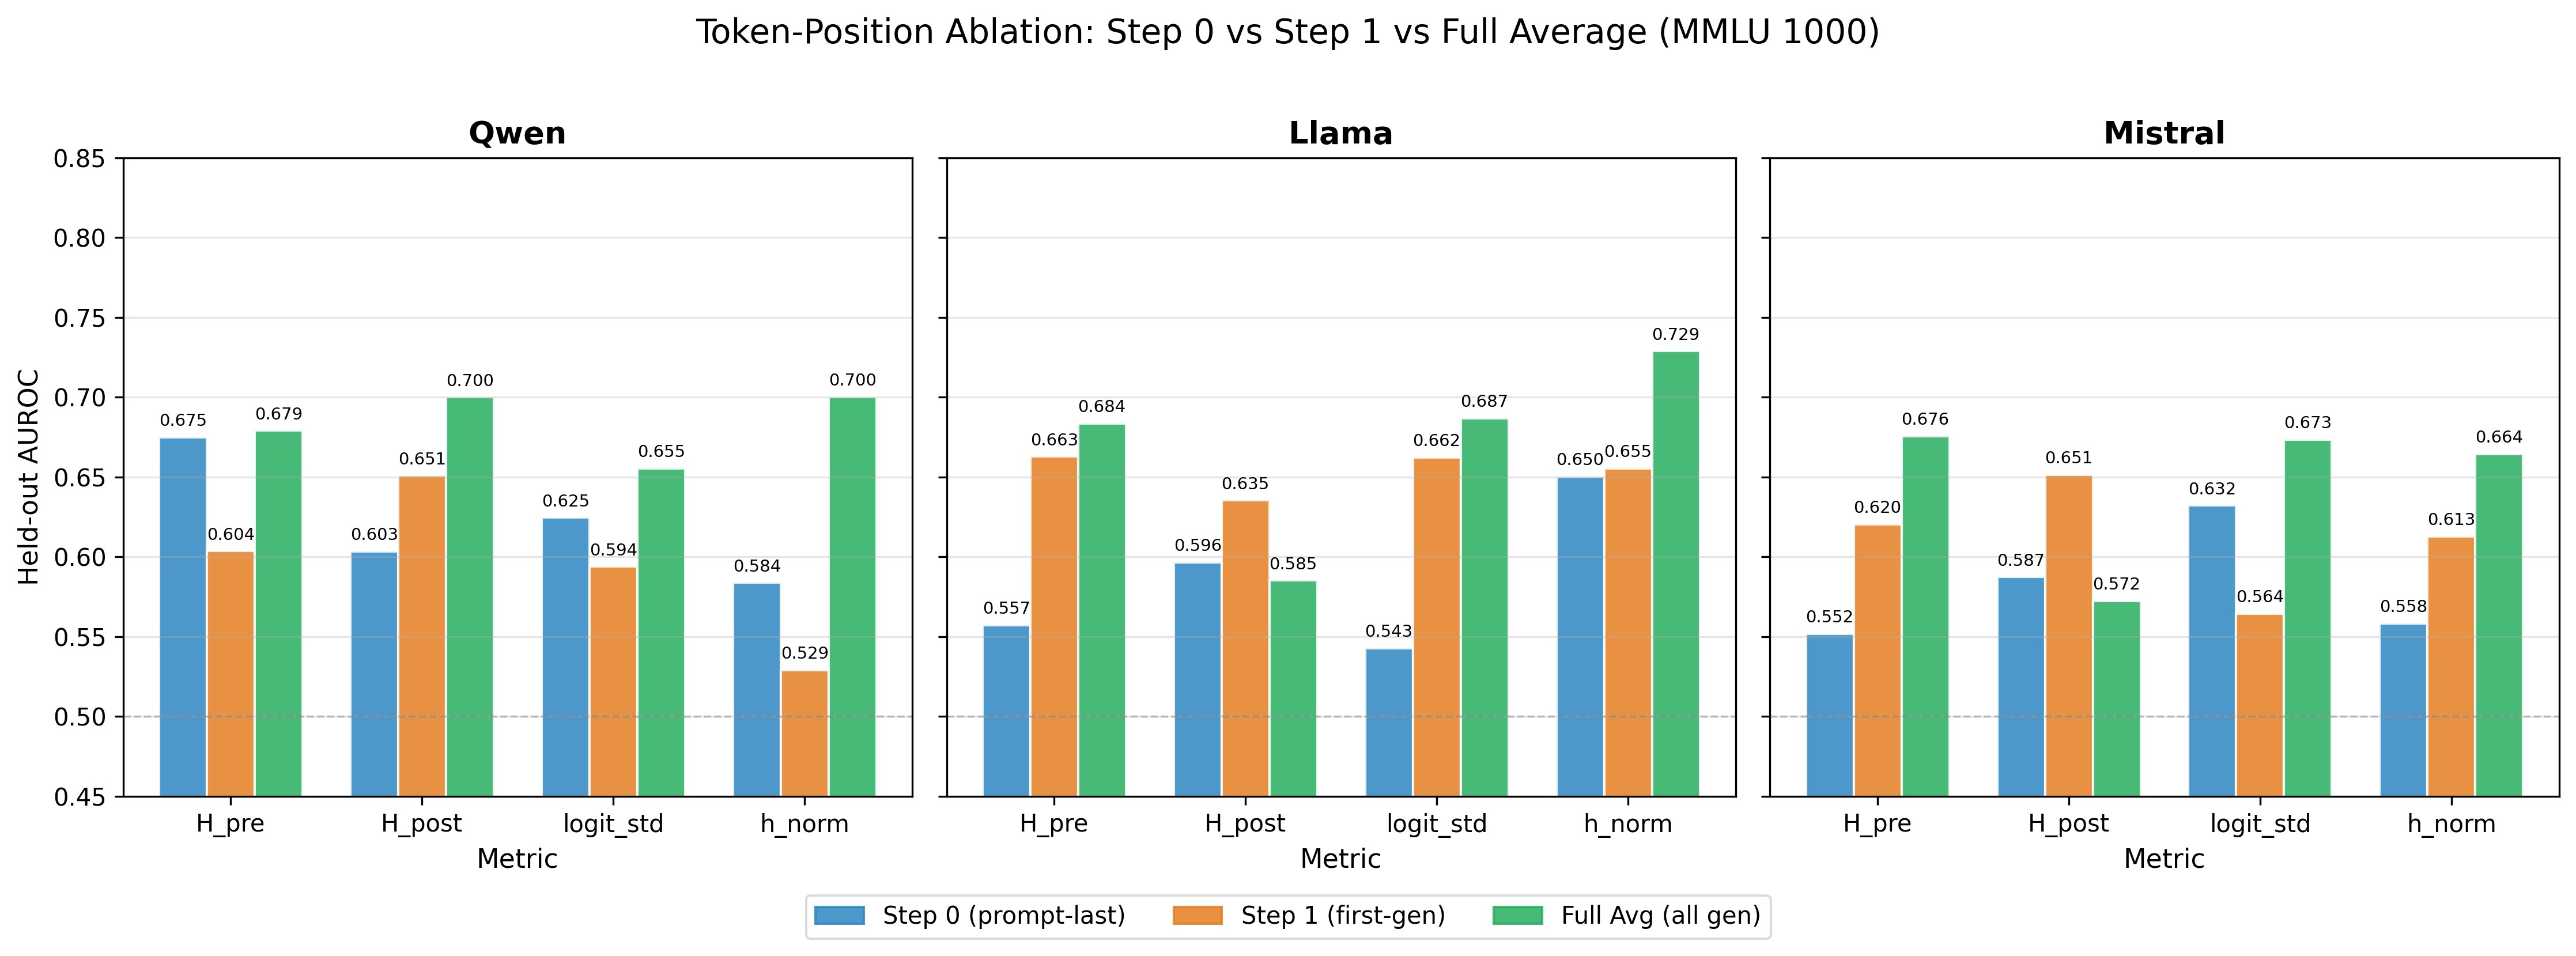
\includegraphics[width=\textwidth]{fig5.png}
\caption{Held-out test AUROC by token position (MMLU, 3 models; independent generation run, not directly comparable to Table~\ref{tab:baseline}). Full-generation average yields the highest AUROC for most metric-model combinations. $\Hpost$ on Llama and Mistral favors Step~1 (first generated token).}
\label{fig:token_position}
\end{figure*}

\FloatBarrier
\section{Reproducibility Protocol Card}
\label{app:protocol}

Table~\ref{tab:master} lists all experimental conditions, protocols, and evaluation parameters.

\begin{table*}[!t]
\centering
\caption{Master experiment table.}
\label{tab:master}
\footnotesize
\setlength{\tabcolsep}{4pt}
\begin{tabular}{l l l c l l l l}
\toprule
Section & Protocol & Dataset & $n$ & Token position & Split & Layer selection & Metric \\
\midrule
4.2 & Scale intervention & Qwen Hard & 500 & Step 0 (prompt-last) & None & All layers & Mean $\Hpre$/$\Hpost$ \\
4.3 & Scale intervention & MMLU (3 models) & 500 & Step 0 & None & All layers & Mean $\Hpre$/$\Hpost$ \\
5.1--5.2 & Baseline evaluation & Qwen Hard / MMLU (3) & 499/1000 & Generation average & 70/30 cal/test & On cal.\ set & Held-out AUROC \\
6.1 & Token-position ablation & MMLU (3 models) & 1000 & Step 0, Step 1, Full avg & 70/30 cal/test & On cal.\ set & Held-out AUROC \\
7.1 & Lens faithfulness & Qwen MMLU & 1000 & Step 0 & 70/30 cal/test & On cal.\ set & AUROC, KL, top-1 \\
7.2 & Classifier comparison & All 4 conditions & 499/1000 & Generation average & 70/30 cal/test & On cal.\ set & Held-out AUROC \\
7.5 & TL control (Step 0) & MMLU (3 models) & 1000 & Step 0 & 70/30 cal/test & On cal.\ set & Held-out AUROC \\
7.5 & TL control (gen-avg) & MMLU (3 models) & 1000 & Generation average & 70/30 cal/test & On cal.\ set & Held-out AUROC \\
7.6 & EL protocol-matched & MMLU (2 EL models) & 1000 & 32 gen tokens avg & 10-fold CV & On each fold & 10-fold CV AUROC \\
5.4 & Deterministic robustness & MMLU (3 models) & 1000 & Gen.\ avg (greedy) & 70/30 cal/test & On cal.\ set & Held-out AUROC \\
5.3 & Multi-seed generation & MMLU (Qwen) & 1000 & Generation average & 70/30 cal/test & On cal.\ set & Held-out AUROC \\
App.~F-E & Task extension & TruthfulQA mc1 (Qwen) & 817 & Generation average & 70/30 cal/test & On cal.\ set & Held-out AUROC \\
\bottomrule
\end{tabular}
\end{table*}

Table~\ref{tab:baseline} reports the five baselines chosen a priori (output entropy, $\Hpre$, $\Hpost$, h\_norm, logit\_std); the full 12-baseline glossary and compact protocol card are provided in the repository. Key protocol parameters are summarized below.

{\sloppy
\textbf{Logistic regression settings (Table~\ref{tab:incremental}, Section~\ref{sec:classifier}):} sklearn LogisticRegression, solver=lbfgs, C=1.0 (default L2), StandardScaler (fit on calibration only), no class weighting, max\_iter=1000.

\textbf{Tuned Lens training (Section~\ref{sec:faithfulness}, Appendix~\ref{app:tuned}):} Per-layer affine translator, wikitext-2 validation, 3 epochs, Adam optimizer, lr=$10^{-3}$, KL divergence loss, final loss \mbox{7009\,$\to$\,2459}.

\textbf{Data provenance.} MMLU: \texttt{cais/\allowbreak mmlu}, config=\texttt{all}, split=\texttt{test}, 1000 items selected via \texttt{np.random.choice} (seed=42). competition\_math: \texttt{qwedsacf/\allowbreak competition\_math}, split=\texttt{train}, Level 4--5 filtered, 500 items (seed=42). ARC: \texttt{allenai/\allowbreak ai2\_arc}, config=\texttt{ARC-\allowbreak Challenge}, split=\texttt{train}. TruthfulQA: \texttt{truthful\_qa}, config=\texttt{mc1}. Model IDs: \texttt{Qwen/\allowbreak Qwen2.5-7B-Instruct}, \texttt{meta-llama/\allowbreak Meta-Llama-3-8B-Instruct}, \texttt{mistralai/\allowbreak Mistral-7B-Instruct-v0.3}. The competition\_math dataset provides only a train split; ARC train was used as a prompt pool. No model fitting on benchmark labels was performed in either case, so train/test leakage does not apply. Exact item manifests are released in the repository.

\textbf{Prompt template (MMLU, 0-shot).} System message: \textit{``You are a helpful assistant that answers multiple choice questions step by step.''} User message: \textit{``Answer the following multiple choice question step by step. $\backslash$n$\backslash$nQuestion: \{question\}$\backslash$n$\backslash$n\{choices\}$\backslash$n$\backslash$nThink through each option carefully, then end with `The answer is [LETTER]' where LETTER is A, B, C, or D.''} Choices are formatted as \texttt{A. \{text\}}, one per line. Chat-template serialization follows each model's default \texttt{tokenizer.apply\_chat\_template}.

\textbf{Answer extraction (MMLU).} Regex priority chain: (1)~\texttt{[Tt]he answer is\allowbreak$\backslash$s*[:$\backslash$s]*\allowbreak$\backslash$(?([A-Da-d])\allowbreak$\backslash$)?}; (2)~\texttt{[Aa]nswer\allowbreak$\backslash$s*[:$\backslash$s]*\allowbreak$\backslash$(?([A-Da-d])\allowbreak$\backslash$)?}; (3)~\texttt{[Tt]herefore\allowbreak ,?$\backslash$s*...\allowbreak$\backslash$(?([A-Da-d])\allowbreak$\backslash$)?}; fallback: last single-letter match. For competition\_math, the final \texttt{$\backslash$boxed\{\allowbreak ...\}} span is extracted. Samples with no valid extraction are excluded.

\textbf{Generation-average entropy.} For each sample and layer~$l$, per-token entropy is computed at every generated token position (including the first generated token; prompt tokens excluded). The generation-average feature is $\bar{H}_l = \frac{1}{T} \sum_{t=1}^{T} H_l^{(t)}$, where $T$ is the number of generated tokens. Output entropy uses the same aggregation at the final layer ($l = L$), ensuring direct comparability with internal-layer features. End-of-sequence (EOS) and padding (PAD) tokens are not explicitly excluded; since batch size is 1 throughout, no padding tokens enter the average. Logits from the \texttt{lm\_head} projection are upcast to FP32 (\texttt{.float()}) before softmax; all subsequent probability, log, and entropy computations remain in FP32. Probabilities are clamped at $10^{-10}$ before log computation. A sample is discarded if entropy values contain NaN at any layer.

\textbf{Cross-validation.} 5-fold and 10-fold analyses use \texttt{StratifiedKFold} (\texttt{shuffle=True}, \texttt{random\_state=42}). For every fold, \texttt{StandardScaler} is fit on the training fold only and applied to the held-out fold.

\textbf{Layer/sign reselection.} Best layer and sign are selected independently for each model $\times$ metric $\times$ protocol combination on the calibration set. Under greedy decoding, selections are made on the greedy calibration split; no selections from the sampled protocol are reused. For each token-position ablation, best layer and sign are selected independently on that condition's calibration split.
}% end sloppy

Detailed multi-layer profile comparisons and self-consistency results are provided in the repository.

\FloatBarrier
\section{Robustness Analysis}
\label{app:repeated}

\subsection{Repeated-Split Analysis}

Table~\ref{tab:repeated} summarizes the repeated-split results. To assess the stability of layer selection, sign selection, and AUROC under different data splits, we repeat the main held-out evaluation protocol 20 times with independent 70/30 stratified splits (seeds 0--19) on all four primary conditions. No model retraining or regeneration is performed; only the calibration/test partition changes.

\begin{table}[!h]
\centering
\caption{Repeated-split summary (20 splits, seeds 0--19). [Protocol: sampled, gen-avg, 70/30 split]}
\label{tab:repeated}
\footnotesize
\setlength{\tabcolsep}{2pt}
\begin{tabular}{l cccc c}
\toprule
Metric & AUROC & std & Layer (freq) & Sign & Range \\
\midrule
\multicolumn{6}{c}{\textbf{Qwen Hard}} \\
\midrule
$\Hpre$ & 0.736 & .047 & L16 (13) & $-$(20) & .624--.830 \\
$\Hpost$ & 0.668 & .057 & L27 (19) & $-$(20) & .475--.745 \\
logit\_std & 0.772 & .031 & L4 (9) & $+$(20) & .703--.833 \\
h\_norm & 0.794 & .031 & L18 (20) & $+$(20) & .751--.862 \\
\midrule
\multicolumn{6}{c}{\textbf{Qwen MMLU}} \\
\midrule
$\Hpre$ & 0.615 & .031 & L18 (7) & $-$(20) & .566--.682 \\
$\Hpost$ & 0.661 & .023 & L27 (20) & $-$(20) & .615--.715 \\
logit\_std & 0.642 & .031 & L18 (7) & $+$(20) & .588--.710 \\
h\_norm & 0.626 & .022 & L27 (10) & $-$(10) & .583--.677 \\
\midrule
\multicolumn{6}{c}{\textbf{Llama MMLU}} \\
\midrule
$\Hpre$ & 0.605 & .039 & L0 (20) & $-$(20) & .507--.670 \\
$\Hpost$ & 0.563 & .029 & L10 (11) & $+$(15) & .508--.611 \\
logit\_std & 0.682 & .026 & L13 (18) & $+$(20) & .640--.732 \\
h\_norm & 0.600 & .037 & L0 (18) & $+$(20) & .492--.654 \\
\midrule
\multicolumn{6}{c}{\textbf{Mistral MMLU}} \\
\midrule
$\Hpre$ & 0.686 & .028 & L0 (13) & $-$(20) & .624--.740 \\
$\Hpost$ & 0.566 & .026 & L5 (9) & $-$(20) & .520--.628 \\
logit\_std & 0.725 & .024 & L13 (11) & $+$(20) & .671--.766 \\
h\_norm & 0.704 & .025 & L13 (17) & $+$(20) & .653--.748 \\
\bottomrule
\end{tabular}
\end{table}

Key findings: (1) $\Hpre$ sign is fully stable under sampled generation (80/80). (2) $\Hpost$ sign = +1 in 15/20 on Llama MMLU; h\_norm on Qwen MMLU shows 10/20 sign stability. (3) Layer selection stability is metric-dependent. (4) logit\_std $>$ $\Hpre$ in 79/80 condition-split combinations.

\subsection{Length Confound Control}
\label{app:length}

After regressing out generation length, $\Hpost$ retains 95--103\% of its AUROC across all four conditions, confirming robustness to length confounds. $\Hpre$ and logit\_std show partial length confounding (retain 71--104\%). Full length-residualization values are provided in the repository.

\subsection{Deterministic Robustness: Greedy Decoding Details}
\label{app:greedy}

Greedy single-layer AUROCs with layer selections are now reported in Table~\ref{tab:greedy} Panel~A. Full greedy profile AUROCs and profile-level redundancy results are provided in the repository.

Under greedy decoding, single-layer sign stability degrades substantially (10--13/20 vs.\ 20/20 under sampled), and layer selection is highly variable. Greedy repeated-split and fold-wise profile comparisons are provided in the repository.


\subsection{Radial/Angular Decomposition}
\label{app:radial}

The divergence between causal scale sensitivity (Section~\ref{sec:qwen_case}--\ref{sec:saturation}: all models show $\Hpre$ collapse under unit-norm removal) and correlational decomposition (Qwen $R^2$ = 0.15, Llama $R^2$ = 0.86, Mistral $R^2$ = 0.83) is not contradictory. Scale can causally determine the absolute level of $\Hpre$ while cross-sample differences are driven primarily by direction. In Qwen, hidden-state norms are large and have limited cross-sample variance relative to directional variation, resulting in low $R^2$ despite high causal sensitivity. In Llama and Mistral, norms have more cross-sample variance, producing high $R^2$. Full decomposition tables with per-protocol CIs and profile-level AUROC by component are provided in the repository.

\subsection{Selective Prediction and Supplementary Robustness}
\label{app:ranking}
\label{app:multiseed}
\label{app:truthfulqa}

\textbf{Cross-normalization layer penalty.} The cost of normalization mismatch is quantified in Table~\ref{tab:landscape} Panel~B (sampled protocol). Under greedy decoding, penalties are similar (Qwen +0.138/$+$0.057; details provided in the repository).

\textbf{Selective-prediction ranking instability.} At 80\% coverage, replacing $\Hpre$ with $\Hpost$ as the abstention criterion changed the top-ranked model in 20/20 sampled-generation splits and 19/20 greedy splits. Coverage-sweep selective-accuracy gaps and detailed ranking tables are provided in the repository.

\textbf{Multi-seed generation robustness.} Across two additional generation seeds (123, 456), profile-level ordering is stable (logit\_std $\geq$ $\Hpre$ in both seeds; $\Hpost$ profile shows the smallest cross-seed variation, diff = 0.005, consistent with scale invariance). Best-layer agreement is 3/4 primary metrics (7/8 across all eight scalars); the sole exception is $\Hpre$. Full multi-seed tables are provided in the repository.

\textbf{TruthfulQA mc1 task extension.} A preliminary TruthfulQA mc1 extension (Qwen, 817 items, single-split) is provided in the repository. Scale redundancy patterns are broadly consistent with the MMLU findings, with slightly higher $\Hpre$ incremental utility (+0.016), possibly due to variable choice counts (2--13 vs.\ MMLU's fixed 4).

\subsection{Protocol-Matched Reproduction Details}
\label{app:reproduction}

Table~\ref{tab:el_repro} reports the reproduction results. We match five key design choices from Ali et al.\ \cite{ali2025entropylens}: (1)~1-shot MMLU prompting without chat template (raw text format), (2)~entropy averaged over exactly 32 generated tokens (prompt-last excluded), (3)~$k$-NN classifier with $k$=3, (4)~10-fold stratified cross-validation, and (5)~logit-based answer extraction (highest probability among \{A, B, C, D\} tokens). Sample selection: 1000 MMLU items sampled with seed=42; the original study does not specify its sampling procedure. Temperature=0.3 with \texttt{do\_sample=True}; the original does not specify decoding temperature.

\begin{table}[!h]
\centering
\caption{Protocol-matched reproduction on Entropy-Lens original models (1-shot, 32 tokens, $k$-NN $k$=3, 10-fold CV).}
\label{tab:el_repro}
\footnotesize
\setlength{\tabcolsep}{3pt}
\begin{tabular}{l cc}
\toprule
 & Llama-3-8B & Llama-3.2-3B \\
\midrule
Accuracy & 62.6\% & 61.5\% \\
$\Hpre$ $k$-NN & 0.549 $\pm$ 0.097 & 0.519 $\pm$ 0.051 \\
$\Hpost$ $k$-NN & 0.578 $\pm$ 0.046 & 0.505 $\pm$ 0.053 \\
$\Hpre$ LR & 0.617 $\pm$ 0.033 & \textbf{0.606 $\pm$ 0.035} \\
$\Hpost$ LR & 0.620 $\pm$ 0.071 & 0.553 $\pm$ 0.044 \\
Scale LR & \textbf{0.668 $\pm$ 0.051} & 0.576 $\pm$ 0.022 \\
Best-layer shift & 19 layers (L1$\to$L20) & 17 layers (L5$\to$L22) \\
\bottomrule
\end{tabular}
\end{table}

Scale profiles outperform entropy on Llama-3-8B; adding $\Hpre$ yields $\delta$=$-$0.001 (scale 0.668). On Llama-3.2-3B, $\Hpre$ LR outperforms scale LR by +0.030 and adding $\Hpre$ to scale yields $\delta$=+0.024---the largest across all models, but in a low-discrimination regime (scale AUROC = 0.576). Classifier switching ($k$-NN to LR) increases AUROC by +0.04 to +0.09. Best-layer shifts: 19 layers on Llama-3-8B ($\Hpre$ L1 $\to$ $\Hpost$ L20), 17 layers on Llama-3.2-3B ($\Hpre$ L5 $\to$ $\Hpost$ L22). Expansion/pruning labels were unchanged between $\Hpre$ and $\Hpost$ on both models.


%===============================================================================
\FloatBarrier

\section*{Acknowledgment}

This work was supported by the Korea Institute for Advancement of Technology (KIAT) grant funded by the Korea government (Ministry of Trade, Industry and Energy) through the International Cooperation in Industrial Technology program (Project Number: P0026190) and Institute of Information \& Communications Technology Planning \& Evaluation (IITP)-Innovative Human Resource Development for Local Intellectualization program grant funded by the Korea government (MSIT) (IITP-2026-RS-2024-00436773). During the preparation of this manuscript, OpenAI GPT-4o and Anthropic Claude were used for iterative manuscript review, claim calibration, reference verification, and language editing. These tools were not used to generate experimental data, analyses, tables, or figures. The authors reviewed and edited all AI-generated suggestions and take full responsibility for the content of this publication.

\bibliographystyle{IEEEtran}
\bibliography{references}

\begin{IEEEbiography}[{\includegraphics[width=1in,height=1.25in,clip,keepaspectratio]{psm.jpg}}]{SUNGMOON PARK} is currently pursuing the B.S. degree with the Department of Healthcare IT, Inje University, Gimhae, Republic of Korea. His research interests include Hyperledger Fabric smart contract security, small language models for code analysis, language model internals and diagnostic measurement, and blockchain-based AI transparency.
\end{IEEEbiography}

\begin{IEEEbiography}[{\includegraphics[width=1in,height=1.25in,clip,keepaspectratio]{yjh.jpg}}]{JINHONG YANG} received the Ph.D. degree in information and communications engineering from the Korea Advanced Institute of Science and Technology (KAIST), Daejeon, Republic of Korea, in 2017. Since 2018, he has been an Associate Professor with the Department of Healthcare IT, Inje University, Gimhae, Republic of Korea. His research interests include agentic AI and physics-informed neural networks.
\end{IEEEbiography}

\EOD

\end{document}
